\documentclass[spanish,english,12pt,letterpaper,oneside]{book}
\usepackage{layout}
\usepackage[spanish]{babel}
\usepackage{calc}
\usepackage[latin1]{inputenc}
\usepackage{graphicx}
\usepackage{subcaption}
\usepackage{latexsym}
\usepackage{amssymb}
\usepackage{fancybox}
\usepackage{fancyvrb}
\usepackage{fancyhdr}
\usepackage{relsize}
\usepackage{pgf,pgfarrows,pgfnodes}
\usepackage{pgfplots}
\usepackage{tikz}
\usepackage{pbox}
\usepackage{rotating}
\usepackage{tabularx}
\usepackage{color}
\usepackage{float}
\usepackage{index}
%\usepackage{wasysym}
\usepackage{indentfirst} %always indent first paragraph after chapter or section
\usepackage{amsmath}
\usepackage{multirow}
\usepackage{notoccite} %avoid citation on list of figures and tables affect order
\usepackage{listings}
\usepackage[pdftex,hyperindex,breaklinks]{hyperref}%,colorlinks,urlcolor=blue,linkcolor=blue]{hyperref}
\usepackage[justification=centering]{caption}
\usepackage[left=4cm,top=3.0cm,right=3.4cm,bottom=3.9cm]{geometry}

%Para activar el doble espacio
%\renewcommand{\baselinestretch}{2} 

\usepackage[ruled]{algorithm}

%\usepackage[noend]{algpseudocode}
\usepackage{algpseudocode}

\usepackage{tcolorbox} 

% new tcolorbox environment
% #1: tcolorbox options
% #2: color
% #3: box title
\newtcolorbox{mybox}[3][]
{
  colframe = #2!25,
  colback  = #2!10,
  coltitle = #2!20!black,  
  title    = #3,
  #1,
}


\renewcommand{\headrulewidth}{1pt}
%\renewcommand{\footrulewidth}{0.5pt}


\newcounter{myfootertablecounter}

\newcommand\myfootnotemark{%
  %\refstepcounter{footnote}%
  \addtocounter{footnote}{1}%
  \footnotemark[\thefootnote]%
}%

\newcommand\myfootnotetext[1]{%
  \addtocounter{myfootertablecounter}{1}
  \footnotetext[\value{myfootertablecounter}]{#1}
}

% from now on, myfootnote has to be used rather than footnote to
% adapt the myfootercounter
\newcommand\myfootnote[1]{%
  \addtocounter{myfootertablecounter}{1}
  \footnote{#1}
}%


\pagestyle{fancy}

\rhead[]{\leftmark}
\lhead[\rightmark]{}
%\lfoot[\thepage]{ATLAS Grid Information System}
\rfoot[ATLAS Grid Information System]{\thepage}
\cfoot{} 


%\renewcommand{\listalgorithmname}{\'Indice de algoritmos}
\renewcommand{\chaptermark}[1]{\markleft{\thechapter #1}}
\renewcommand{\sectionmark}[1]{\markright{\thesection #1}}
\renewcommand{\chaptermark}[1]{\markboth{\chaptername \ \thechapter. #1}{}}

\newcommand{\contrib}[3]{#1\quad$<$\texttt{#2}$>$%
{\small\\\quad\textit{#3}}\\[1ex]}

\pgfdeclareimage[width=5cm]{logo-utfsm}{images/logo-grande}

\title{3D Scene Reconstruction}

\author{
  Juan Reyes \\ \texttt{jareyes@alumnos.inf.utfsm.cl}
}

\date{$\infty$}

\frenchspacing

\makeindex

\begin{document}
    \newenvironment{dedication}
        {\vspace{6ex}\begin{quotation}\begin{center}\begin{em}}
        {\par\end{em}\end{center}\end{quotation}}

\frontmatter

\thispagestyle{empty}

\begin{center}

{\large\bfseries Universidad T�cnica Federico Santa Mar�a}\\[2mm]
{\large\bfseries Departamento de Inform�tica}\\[2mm]
\pgfuseimage{logo-utfsm}
\end{center}

\vspace*{\stretch{3}}

\begin{center}
{\LARGE\bfseries 3D Scene Reconstruction }\\[2mm]
{\LARGE\bfseries AAAA}
\end{center}

\vspace*{\stretch{5}}

\begin{center}
{\large por}\\[2mm]
{\huge Juan Alfonso Reyes L�pez}
\end{center}


\vspace*{\stretch{5}}

\begin{center}
{\large Tesis para optar al t�tulo y grado de}\\[2mm]
\vspace*{10mm}
{\Large Ingeniero Civil en Inform�tica}\\[2mm]
{\LARGE Mag�ster en Ciencias de la Ingenier�a Inform�tica}\\[2mm]
%{\large for the degree of}\\
%{\Large Master in Science of Informatic Engineering}
\end{center}

\vspace*{\stretch{5}}


\begin{center}
{\large Valpara\'{i}so, Chile}\\
{\large July, 2013}\\[2mm]
\end{center}

\vspace*{\stretch{1}}

\pagebreak

\thispagestyle{empty}

\begin{center}
{\Large Universidad T\'{e}cnica Federico Santa Mar\'{\i}a} \\
{\Large Departmento de Inform�tica}\\
{\Large Valpara\'{\i}so - Chile}\\
\end{center}

\vspace*{\stretch{1}}

\begin{center}
{\large TITULO DE LA TESIS:}\\
{\large \textbf{3D Scene Reconstruction AAAAA}}
\end{center}

\vspace*{\stretch{1}}

\begin{center}
{\large AUTOR:}\\
{\large \textbf{Juan Alfonso Reyes L�pez}}\\
\end{center}

\vspace*{\stretch{2}}

{\large TRABAJO DE GRADO, presentado en cumplimiento parcial de los
requisitos para el t�tulo de Ingeniero Civil en Inform�tica y el Grado de
Mag�ster en Ciencias de la  Ingenier�a Inform�tica de la Universidad T�cnica Federico
Santa Mar�a.}

\vspace*{\stretch{5}}

\begin{table}[ptbh]
\begin{tabular}[c]{lc}
{\large Prof. Dr. Luis Salinas} & \begin{picture}(200,5) \line(1,0){200} \end{picture}\\
& {\large Profesor Gu�a } \\
& \\
& \\
& \\
{\large Prof. } & \begin{picture}(200,5) \line(1,0){200} \end{picture} \\ 
& {\large Correferente } \\
& \\
& \\
& \\
{\large Dr.} & \begin{picture}(200,5) \line(1,0){200} \end{picture}\\
& {\large Correferente Externo }
\end{tabular}
\end{table}

\vspace*{\stretch{1}}

\begin{center}
{\large Valpara\'{\i}so - Chile. \\ Julio 2013.}
\end{center}
 
\pagebreak


\endinput


\begin{dedication}
A mi madre por inculcarme la importancia de la educaci\'on,

A mi padre por demostrarme la belleza de la creatividad,

A mi hermana por su apoyo incondicional,

A Carolina por compartir su vida conmigo.
\end{dedication}



\chapter*{Abstract}

In general a 3D reconstruction system has three main steps: data acquisition, registration and reconstruction. During the registration step the 3D points are registered to a common coordinate system. The Iterative Closest Point (ICP) algorithm is widely used to perform registration, however it 
is computationally expensive and susceptible to local minimum. This thesis proposes to address these issues, 
applying a filtering step where only edges that appear 
in the two point clouds to be aligned pass the filter. For this purpose a combination of visual and geometrical information is 
used along with the ICP
  algorithm and a pose graph optimization method. The proposed technique reduces the amount of calculations 
involved, because only between 10\% and 20\% of original points are used as input for the ICP algorithm, increasing 
the quality of the alignment, working with the most representative subset of the data. At difference to other techniques 
involving edge filtering along with ICP, this proposal increments the odds of a correct alignment filtering out non common 
data from the pair of point clouds to be aligned. Quantitative results shows the advantages of the proposed method. A 
public available dataset was used, 
providing the source 
code and all the necessary information to compare and replicate the presented results.

\section*{Keywords}

3D reconstruction, simultaneous location and mapping, iterative closest point, Kinect, point cloud



\chapter*{Resumen}

En general un sistema de reconstrucci\'on 3D tiene tres pasos principales: adquisici\'on de datos, registro y reconstrucci\'on. Durante el paso de registro los puntos 3D son registrados en un sistema de coordenadas com\'un. El algoritmo de b\'usqueda iterativa de puntos cercanos (ICP) es 
ampliamente usado para realizar el registro de los puntos, sin embargo es computacionalmente costoso y propenso a converger a un m\'inimo local. Esta tesis propone enfrentar estos problemas, aplicando un paso de filtrado donde solo los bordes que aparecen en las dos nubes de puntos 
que est\'an siendo alineadas pasan el filtro. Una combinaci\'on de informaci\'on visual y geom\'etrica es 
usada junto con ICP y un m\'etodo de optimizaci\'on de grafos. 
La t\'ecnica propuesta 
disminuye la cantidad de c\'omputos necesarios porque s\'olo entre un 10\% y un 20\% de los puntos originales son usados 
como entrada para el algoritmo ICP, 
aumentando la calidad de la alineaci\'on, trabajando con el subconjunto de datos m\'as representativo. A diferencia de otras 
t\'ecnicas que involucran filtrado de bordes junto con ICP, esta propuesta incrementa las probabilidades de una alineaci\'on 
correcta quitando los puntos no comunes entre el par de nubes de puntos a alinear. Los resultados cuantitativos muestran 
las ventajas del m\'etodo propuesto. Un conjunto de datos p\'ublicamente disponible fue utilizado para los experimentos, el c\'odigo 
y toda la informaci\'on necesaria para comparar y replicar los resultados es provista.


\section*{Palabras clave}


Reconstrucci\'on 3D, localizaci\'on y mapeo simult\'aneo, algoritmo de b\'usqueda iterativa de puntos cercanos, Kinect, nube de puntos.


\addcontentsline{toc}{section}{\contentsname}
\tableofcontents

%\addcontentsline{toc}{subsection}{\listalgorithmname}
%\listofalgorithms
\addcontentsline{toc}{subsection}{\listfigurename}
\listoffigures
\addcontentsline{toc}{subsection}{\listtablename}
\listoftables

\mainmatter

\chapter{Introduction}
\label{introduccion}
\index{Introducction}
\indent The 3D scene reconstruction problem consists of taking the
necessary information from a real scene in order to reconstruct
it in a three dimensional space, usually to be displayed 
in a computer. 

The goal is to represent in the most accurate way the geometric scene details, obtaining rich 
information about the scene that is not explicitly contained in a single image, and then use this 
to reconstruct the scene or to perform a more advanced task that depends on the scene geometry. 
3D scene reconstruction has several applications, for example in the field of autonomous robot navigation it is crucial to have 
the scene geometry in order to locate paths, obstacles and know current robot location, this problem is known as 
Simultaneous Localization and Mapping (SLAM) \cite{SLAM06}. Another application of 3D scene reconstruction is augmented reality, 
where a virtual 3D object is added to a real video of the scene. 3D scene reconstruction is also useful in parts inspection 
in a manufacturing plant, where it is necessary to detect
 fabrication defects on some objects, another application is in statues and buildings preservation, in order to have a digital representation 
of the objects and being able to reproduce or maintain them. There are many areas where 3D scene reconstruction is important \cite{apps2009}.

 
In general the information is acquired
 from the scene with optical devices, such as RGB cameras or depth sensors.
Most of 3D scene reconstruction methods can be classified into passive methods and active methods \cite{lanman}.
Passive methods works without controlling the light in the scene, the sensors used by these methods just receive light (ordinary cameras). 
On the other hand, active methods alter the light in the scene, with a light transmitter and its corresponding 
receptor, projecting patterns of light in order to simplify the matching process prior to the triangulation. 
There are also some active methods that touch the object in order to reconstruct it, but they are beyond 
the scope of this thesis. 

Accurate and expensive equipment to perform 3D scene reconstruction are commercial laser scanners,
 but nowadays there are emerging cheaper devices that 
potentially could perform 
a similar reconstruction at a lower cost \cite{kinectReview13}.

One of the most classical approaches to perform 3D reconstruction is to use multiple 2D
 images taken from similar camera viewpoints and estimate the distance of each
 relevant pixel with triangulation (Stereo Vision, Multiview Vision), with these 
approaches the depth map must be generated using the geometrical information contained
 in the images \cite{Newcombe10livedense}. Nowadays, it is common to find devices that generate depth maps accessible
 to everyday users, automating the depth map generation step, these devices are called depth sensors. 
Depth sensors give to each pixel of the image a depth value, related
with the distance of the real object from the sensor, offering  more
accurate data to perform 3D reconstruction. With the appearance
of cheap depth sensors for gaming and entertainment, there is a growing interest in the development of low cost
3D reconstruction systems. 


\section{Goal of the Thesis} 

One of the key steps of a 3D reconstruction algorithm is the registration, where the 3D points corresponding to
 the scene are  registered into a common coordinate system, preserving the original scene disposition. This step is 
 fundamental in order to being able to reconstruct the scene or recover the sensor trajectory.

The goal of this thesis is to propose a new algorithm to register point clouds in a common coordinate system, applying 
filtering to the data and combining visual with geometrical information, in order to obtain better results with less 
computational costs. 






When an scene is beign scanned with a Laser, Time of Flight Camera, structured 
light sensor or other device capable of obtain a depth map of the scene.
 A set of 3D points is obtained per capture, its 3D coordinates 
are relative to the scanning device. Its necessary to move the captured points, 
according to the device movement or rotation, for this reason 
one of the first fundamental steps to reconstruct a 3D scene is the 
positioning of the 3D points on a common coordinate system, conserving 
the original scene structure. 

This problem becomes trivial if we know the device position and orientation 
for each capture or if we have a pair of matches between each two sucesive 
captures. But this not occur in practice and additional problems arise due 
to the noise and imperfections of the device.


In general, when the sensor is collecting the 3D points from the scene, 
 its necessary to move or rotate it in order to capture new objects and surfaces from 
the scene, adding more information to the reconstructed scene. But in order to be 
able to infer the correct position of each capture, is necessary to have part 
of the view in common between two captures (an overlaping area). Thus is posible to position a new capture with respect to an old one in the scene, using this overlaping 
area to correctly align both captures.
 
The overlaping areas of the different captures of a scene must be correctly 
aligned when registering the points in a common coordinate system, 
thus with each new capture more information is added to the scene, 
getting closer to the desired result. 

\subsection{Mathematical definition}

A point cloud is a set of 3D euclidean space points and the problem of aligninig several point clouds 
in order to form a complete 3D model, where intersecting areas overlap perfectly 
is known as registration. Assumming that all point clouds form part of a 3D global model and they can be 
 positioned  consistenly accord to this model.

Let  ${a_i},{b_i} \in \mathbb{R}^3;i = 1,2,...,N$ be two sets of 3D euclidean space points.

We want to find $R,\vec{t}$ that minimizes the following expression:
$$
\sum\limits_{i=1}^N || Ra_i - b_i - \vec{t} ||
$$

Where $R$ is a  $3x3$ rotation matrix and $\vec{t} \in \mathbb{R}^3$ is a translation vector.


In the case that the two sets are identical, the previous expression will have a minimum at zero.

We are interested in applying this minimization scheme to real life data, specifically to consecutive 
point clouds (with very small rotation and translation), in order to register a global 3D model of 
a real scene. In order to beign able to align this point clouds, it is necessary to have an important overlapping 
area which is equivalent to have a very small rotation and translation of the sensor registering the point clouds, 
because this area will allow to minimize distances between paris of points corresponding to the same real world position.


\begin{figure}[!h]
\begin{center}
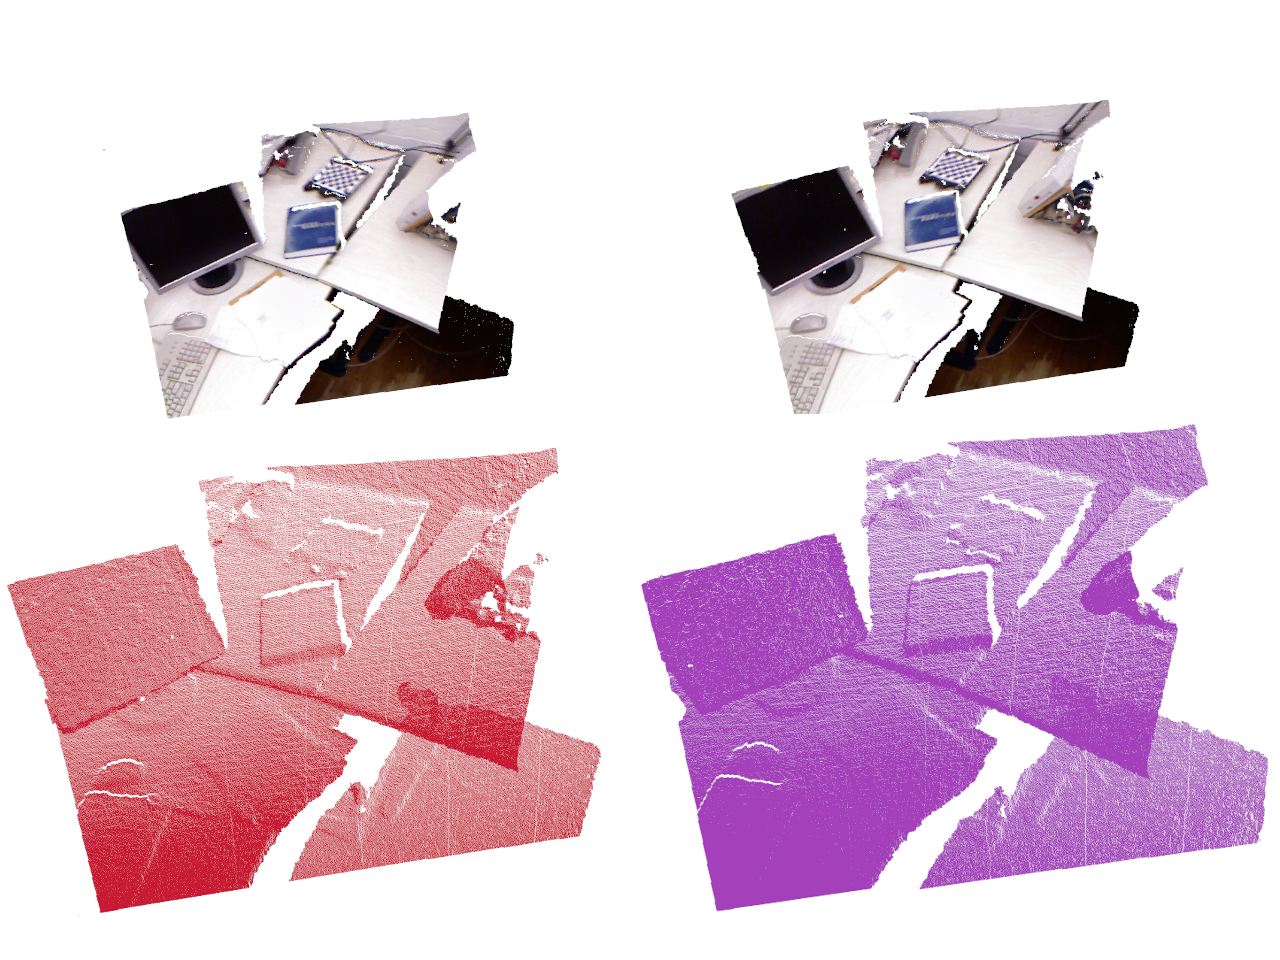
\includegraphics[scale=0.35]{images/two_clouds}
\caption{Two point clouds corresponding to a real life scene. We want to find the correct rotation and translation to align both point clouds.}
\end{center}
\end{figure}


\section{Thesis Outline}

The rest of the document is structured as follows:

\begin{itemize}
\item Chapter 2: Presents recent and important works in 3D reconstruction. 

\item Chapter 3: Explains the sensor used to capture the data and how it works.

\item Chapter 4: Describes all the used techniques and the proposed method.

\item Chapter 5: Presents the dataset, tools and results obtained with the proposed method.

\item Chapter 6: Presents the conclusions and the future works.
\end{itemize}

\chapter{State of Art}
\index{State of Art}
 
Nowadays there is a growing interest on the 3D scene reconstruction field, due to the incresing computational power and the reduction of 
the costs of the capturing devices. There are a lot of differents approaches to afront the problem, there are works that perform 3D reconstruction 
from a video, from a set of images taken with an unknown camera and orientation, using active devices that project patterns of light into 
the scene, lasers, etc. 

In 3D reconstruction an important part of the problem depends of the intrinsical 
device characteristics (noise, resolution, framerate, etc), the scene or object beign captured, ilumination, the camera location and position, etc. All this factors configure different instances of the problem, difficulting the comparison and limiting the use of a common dataset, but some efforts in order to allow comparison between different algorithms has been made 
in \cite{seitz2006}, \cite{ponce2006} and \cite{scharstein2001}.

The researchers can estimate their systems performance comparing the generated 3D model with some 
ground truth model obtained with a high precision laser scanner, but not always is possible to have a ground truth model, because lasers scanners 
are expensive equipments. Due to this its common to measure the performance
 comparing some result obtained at an intermediate step of the reconstruction process with a ground truth measure, 
such as the camera estimated path with camera real path.   

%done
Reconstruction from a set of photographs without human assistance is performed in \cite{jan}, they demonstrated the first system able to deliver dense geometry for Internet scale photo collections with millions of images of an entire city within the span of a day on a single PC. They used appearance-based clustering in multiple CPU and GPU cores 
in order agrupate images corresponding to the same site, using gist features for each image along with a RGB
descriptor in order to mantain color information. They also used geo-location information available for some of 
the images. Then at each cluster they performed 3D reconstruction using only the images with mutually consistent epipolar 
geometry. From millions of images from one city they generated thousands of 3D models of buildings. See figure \ref{fig:jan}. 


\begin{figure}[h!]
\begin{center}
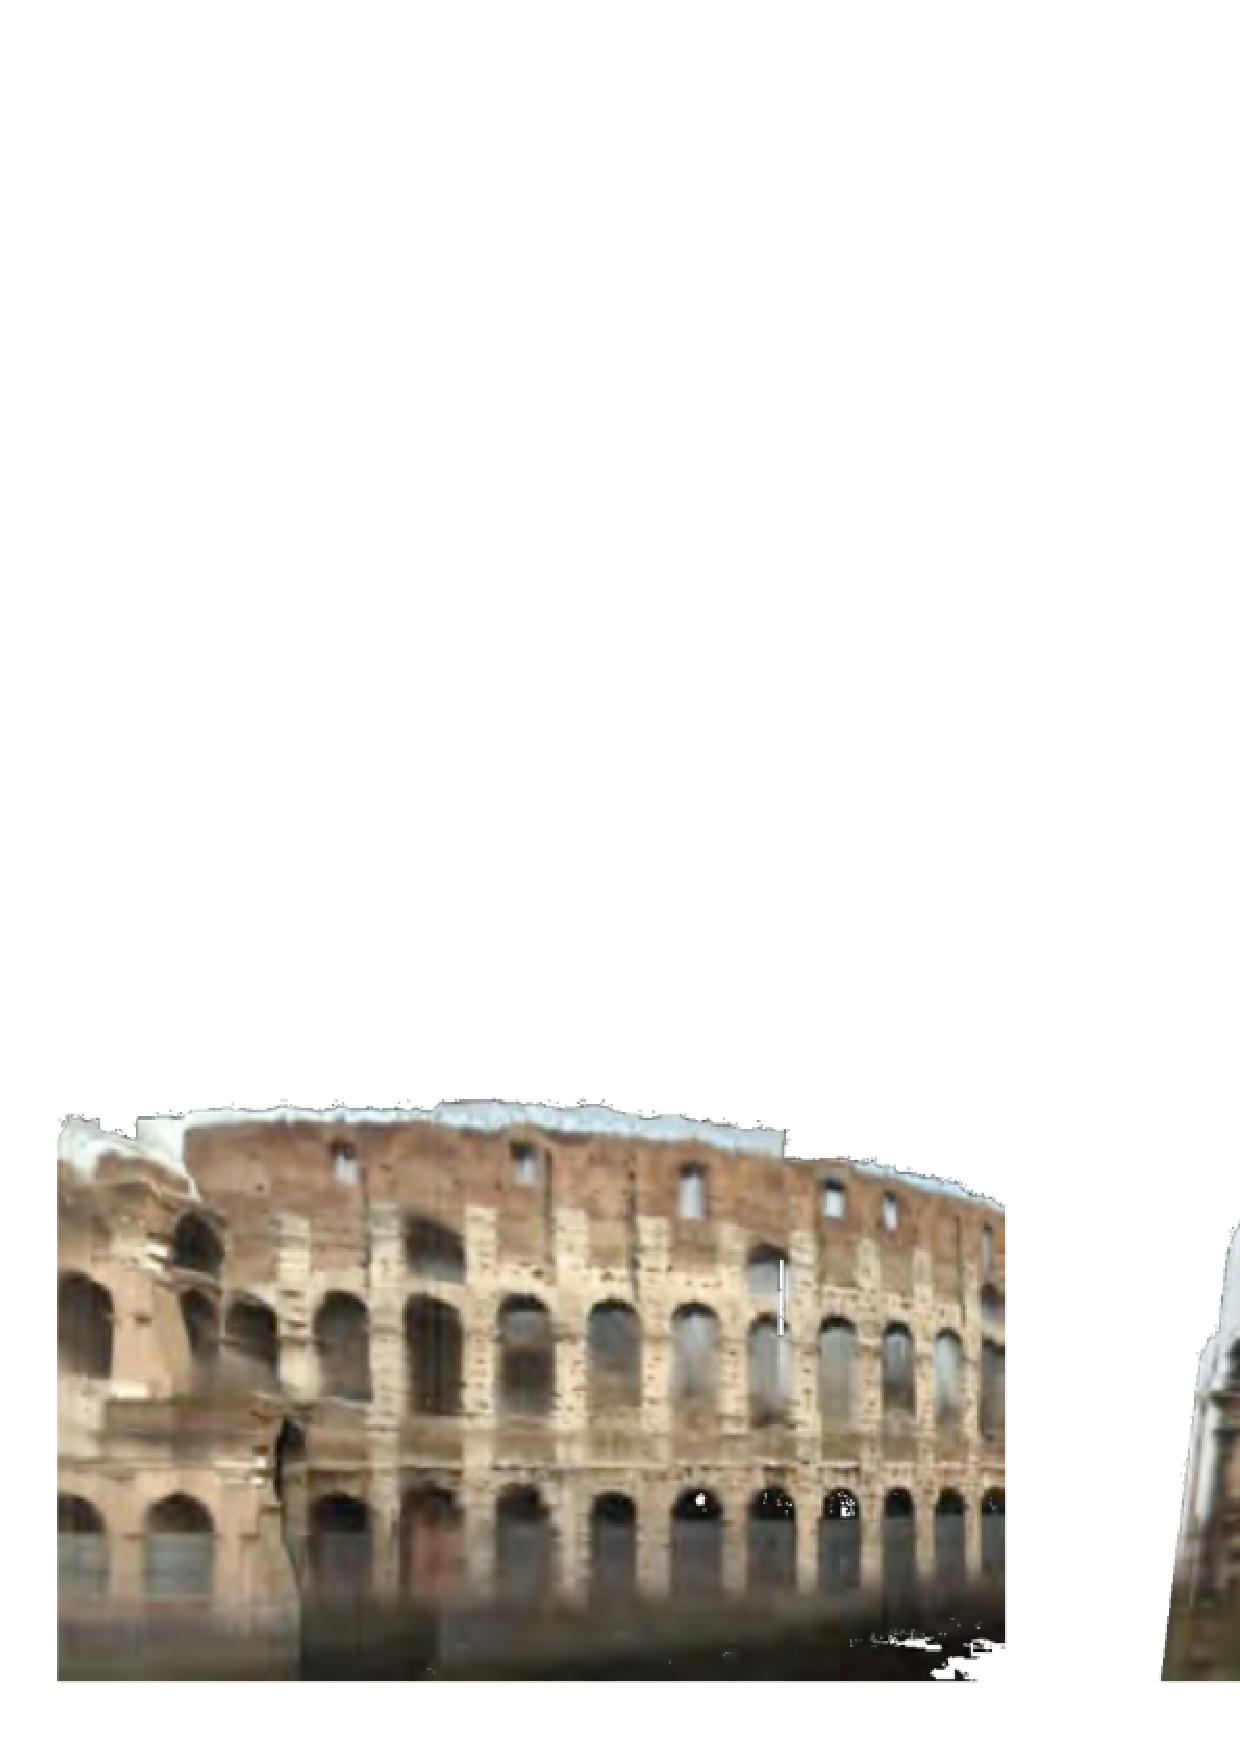
\includegraphics[scale=0.25]{images/jan}
\caption{Reconstructed 3D buildings in less than 24 hr. using 2.8 million and 2.9 million of images respectively}
\label{fig:jan}
\end{center}
\end{figure}

%done
In \cite{guangyu} an hybrid approach is used, combining a ToF (Time of Flight) camera and an grayscale camera in order to perform the reconstruction. 
The data adquisition is made rotating the object in front of the camera with a black background behind it, then they use 
SIFT (Scale Invariant Feature Transform) to find 2D feature correspondences and perform and initial alination between two consecutive frames, this alineation is 
then improved with ICP (Iterative Closest Point) algorithm. They use a 3D laser scanner in order to obtain a ground truth, obtaining a difference around of 1\% 
between their reconstructed
 models and the 3D laser models. See figure \ref{fig:guangyu}.




\begin{figure}[h!]
\begin{center}
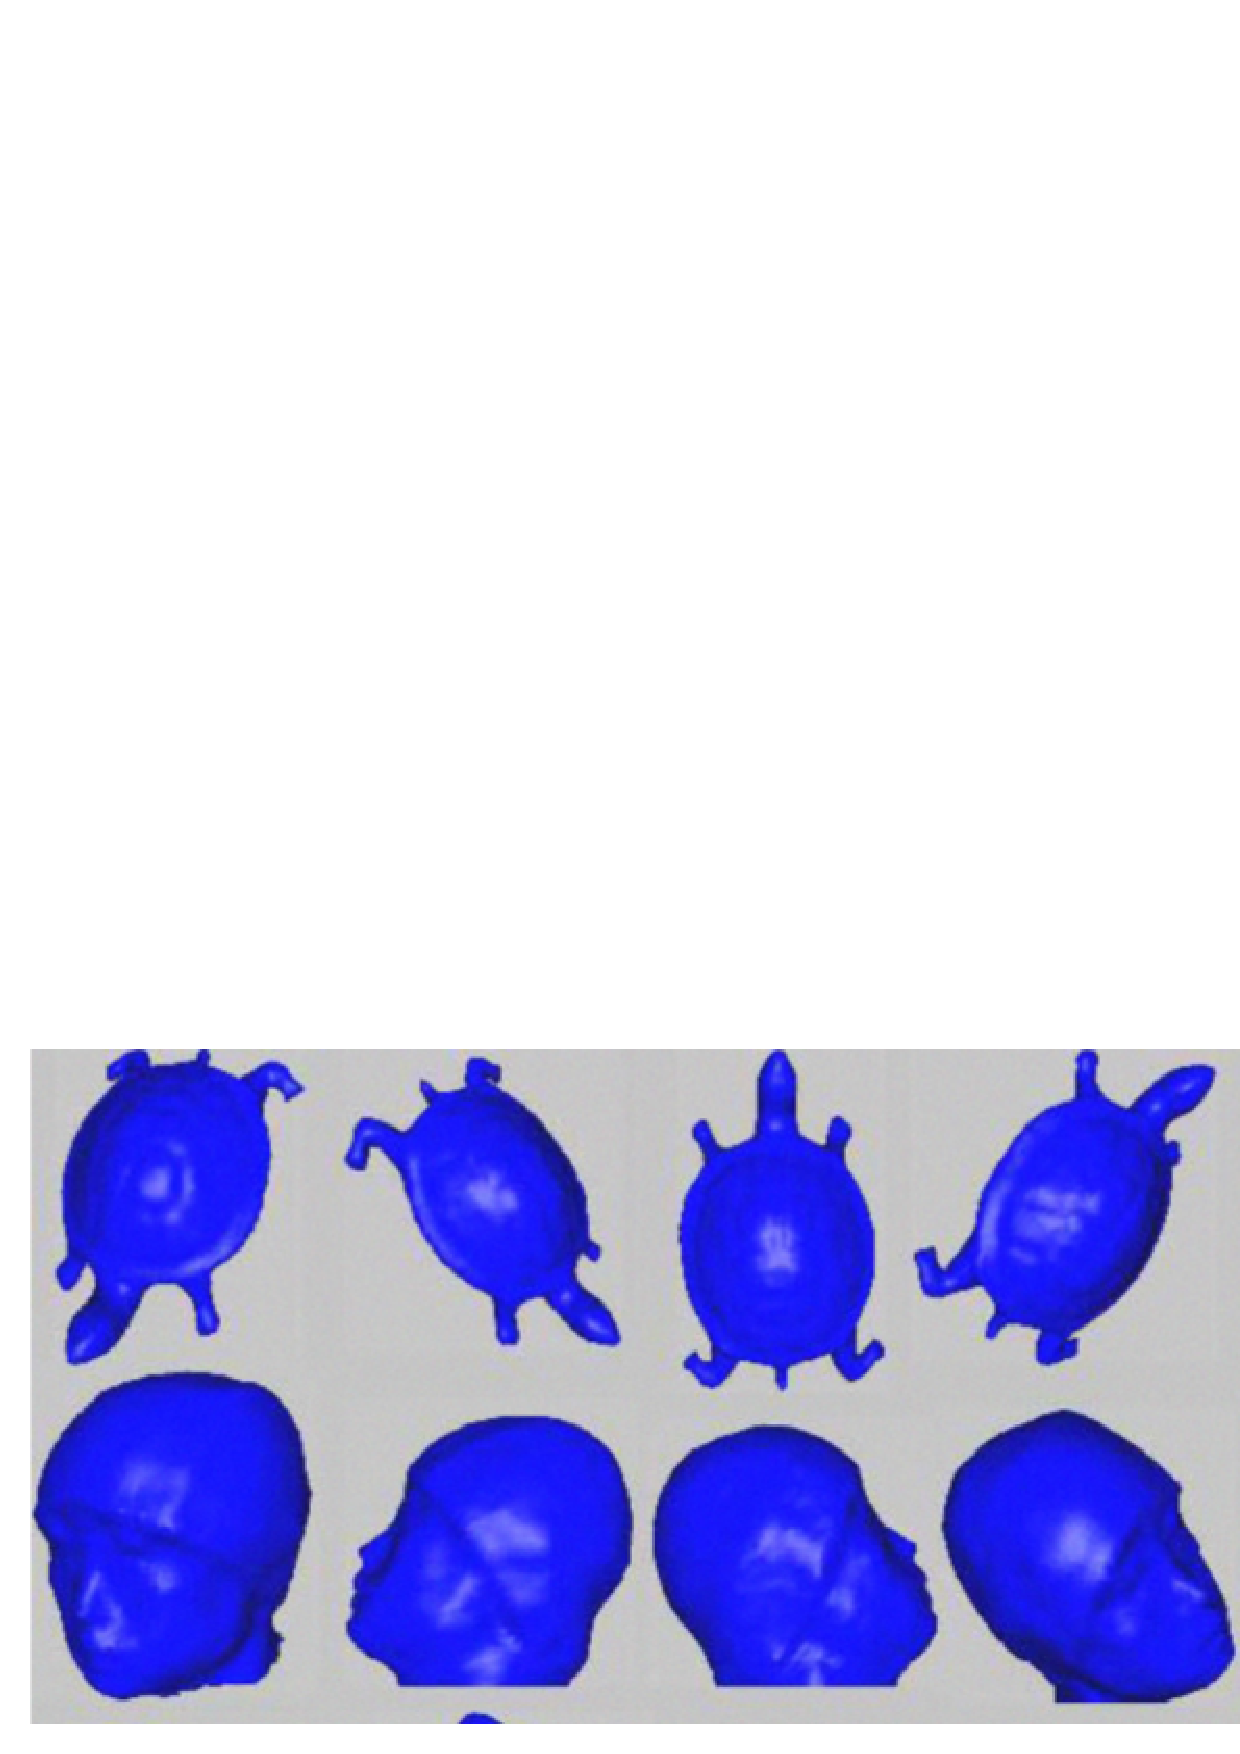
\includegraphics[scale=0.38]{images/guangyu}
\caption{3D Reconstruction of a human head and an object using ToF and RGB camera}
\label{fig:guangyu}
\end{center}
\end{figure}

%done
In \cite{may2009} a ToF camera is used in combination with an industrial robot arm (KUKA KR 16) in order to register an indor scene,
they use an improved version of the ICP algorithm called ICP Frustum, where at each iteration the points that are not overlaping with the previous frame are removed. The industrial robot arm is used to move the camera and get a ground truth camera path to evaluate the performance of their ICP algorithm. 

%Its possible to find more elaborated reconstructions using a laser scanner, but its a more expensive method. In 
%\cite{binney} there is a interesting work where a reconstruction of tree branches is performed using a laser range 
%data. They use a probabilistic approach and use knowledge about the tree structure to guide an iterative reconstruction 
%process. 

%done
In \cite{keqiang} a 3D reconstruction is performed with a laser range finder (SICK 2D ) and a mobile robot, 
using the ICP algorithm and a volumetric representation. In the matching phase of the ICP algorithm not all
 points are used, instead they just use edge points, reducing the computational cost of the process. The scene 
 representation is simplyfied removing redundant points, this is done dividing the scene into voxels and at each 
 voxel preserving just the point closer to the center. Their system produces a scene with data points evenly 
 distributed.

%revisar nuevamente
In \cite{wei} a CCD camera and a 2D laser scanner is used to perform indoor panoramic 3D reconstruction, 
they mounted both devices in a rotational stage and use a fusion algorithm to merge the depth map generated by the laser 
and the depth map generated from the CCD camera observations, the two depth maps contains noise and an intelligent merging reduce this
 noise giving more accurate information to the 3D reconstruction process. Another interesting work of indoor scene reconstruction is \cite{henry} where an RGB-D camera is used to reconstruct an indoor scene. RGB-D cameras are sensing systems that capture RGB images
 along with per pixel depth information. They use the ICP algorithm to calculate the camera location and pass to it information from 
the depth camera and  rich visual
 features along with RANSAC (RAndom SAmple Consensus) verification captured by the RGB camera. They use surfels \cite{pfister} to represent the scene. See figure \ref{fig:henry}.

\begin{figure}[h!]
\begin{center}
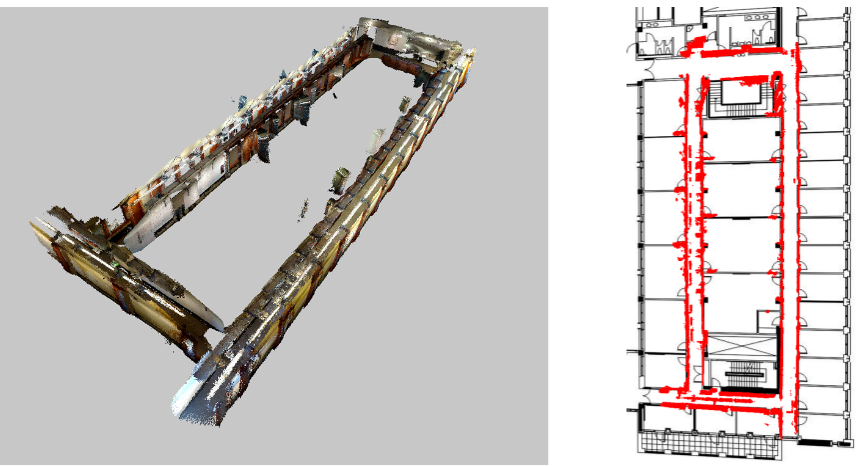
\includegraphics[scale=0.29]{images/henry}
\caption{Reconstructed 3D big indoor space}
\label{fig:henry}
\end{center}
\end{figure}

%done
In \cite{cui} a ToF camera is used to reconstruct 3D objects. A combination of 3D superresolution method with a 
probabilistic scan alignment (iterative Expectation Maximization) approach that takes into account the sensor's 
noise characteristics is used. Their method is not in real time and the resulting models contains undesirable 
artifacts due to  the noise of the captured depth maps, they use a low resolution device (176x144) and they 
improve the resolution using a superresolution method. They captured a ground truth model with a laser 3D scanner, 
obtaining differences below 1 cm in most areas between their model and the ground truth model. Their scanning 
procedure doesn't allow a freely movement around the object, the object must be at the center of view of the camera 
and the distance between the object and camera must be almost constant. A similar work can be found at \cite{schoun} where 
 a hierarchical Lukas Kanade optical flow is used for registration.
 
see figure \ref{fig:cui}.

\begin{figure}[h!]
\begin{center}
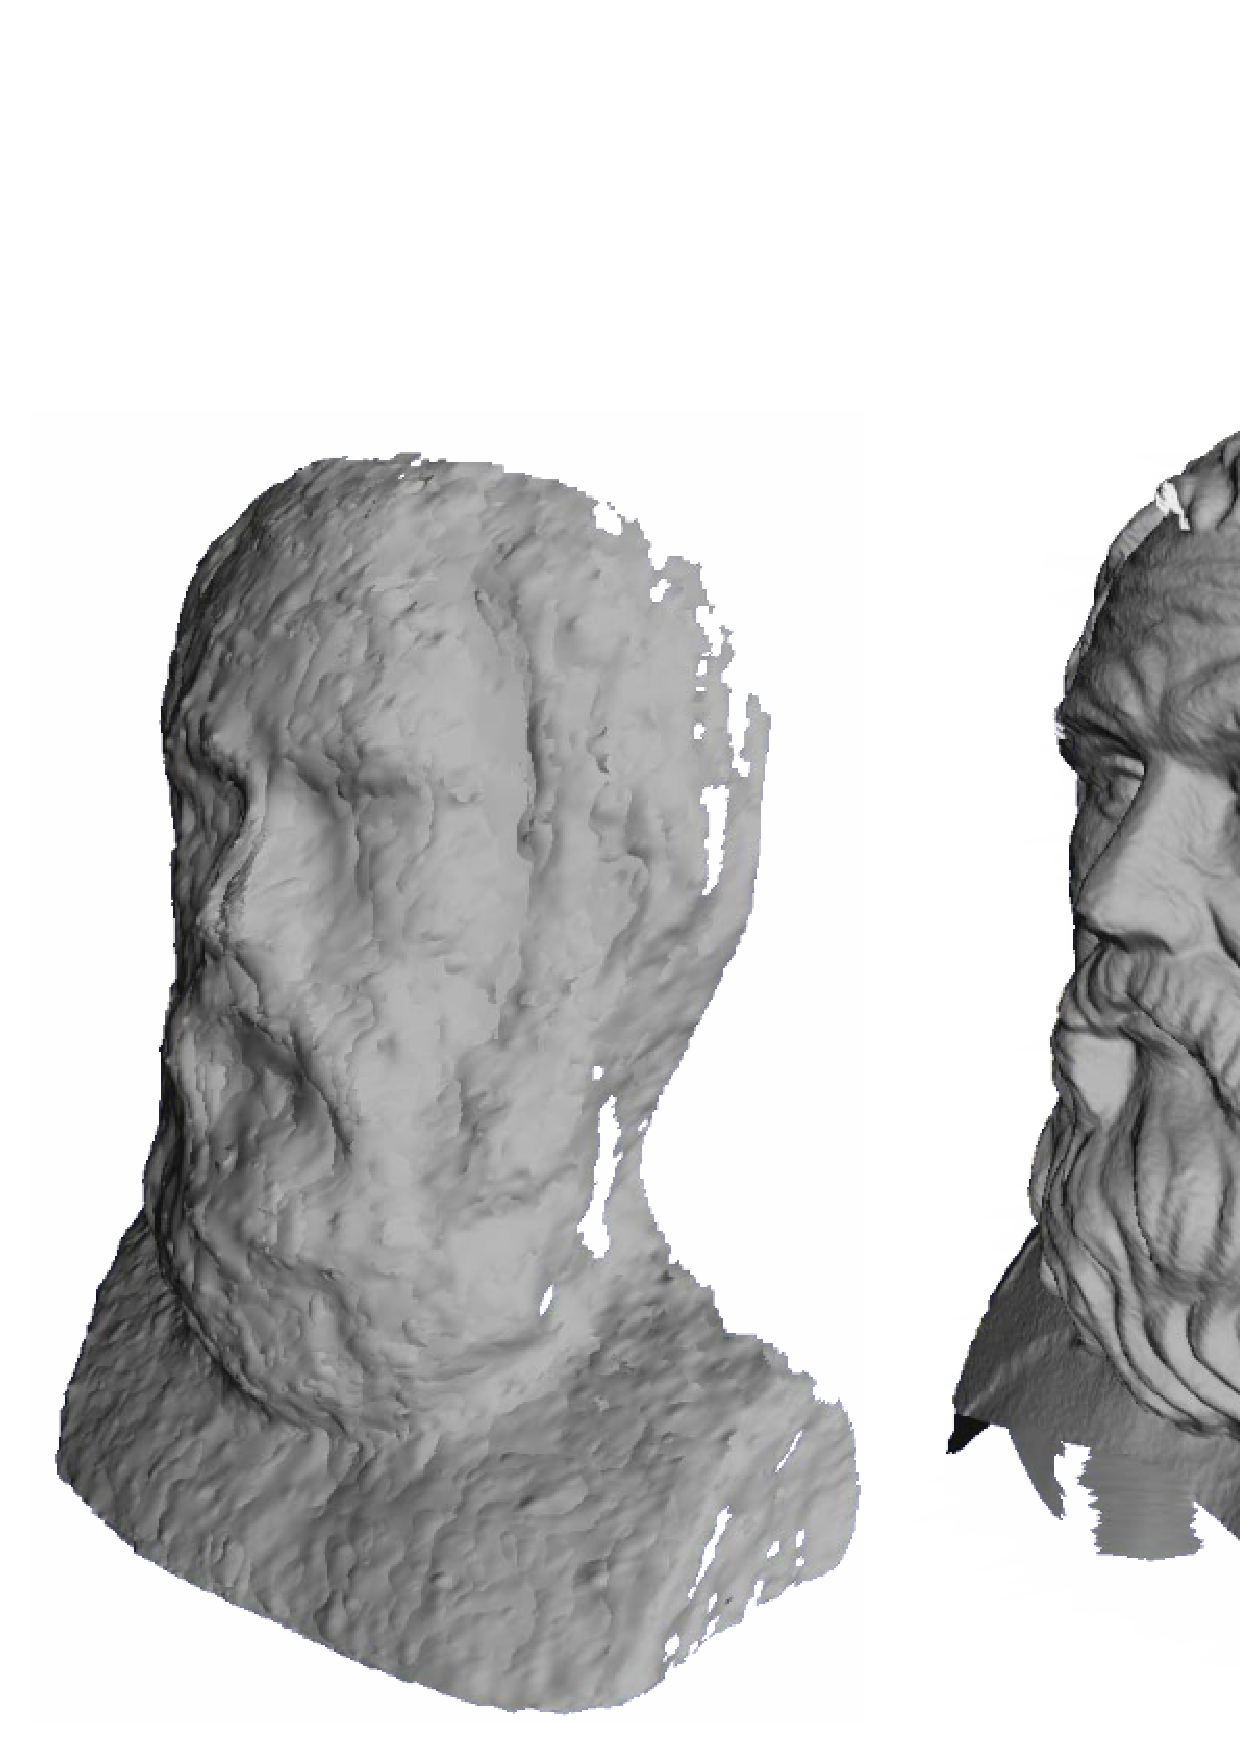
\includegraphics[scale=0.23]{images/cui}
\caption{ToF Reconstruction, Laser Reconstruction and Error Plot}
\label{fig:cui}
\end{center}
\end{figure}

In \cite{huhle} a ToF camera and a RGB camera are used generate a 3D model, they combine geometric and color information, 
using SIFT to determine matching features between the RGB images, 
this 2D points are then converted into 3D points using the depth information. They use  Normal Distributions Transform (NDT) \cite{biber03} to exploit the geometrical 
information. NTD is a registration algorithm that use a different principle than ICP, it doesn't need point matches 
between sucesive frames. NTD build a grid on the 2D depth image, calculating the mean and the covariance matrix for each 
 cell. The respective normal distributions are used to estimate the probability of any transformed point $T(x_i)$ to fall 
inside some cell. Then they define a function that depends on the RGB matching features and NTD, in order to find the desired 
rigid transformation.

 
%done
A very interesting work is made in \cite{izadi}(figure \ref{fig:izadi}), they use a low cost RGB-D camera (Kinect) in order to perform
the 3D reconstruction using the ICP algorithm  and a volumetric representation with a GPU in order to 
archieve real time reconstruction. The camera can move freely around the scene and the reconstruction grows in detail 
as new depth measurements are added. They apply color textures to the reconstructed scene obtaining very 
realistic models, their system is able to perform rigid body collisions 
simulations during the reconstruction, allowing thousands of virtual particles interact with the scene. Also a 
user can interact with the scene during the reconstruction process. This is one of the most advanced 
reconstruction systems, due to its uniques features. A precursor work of \cite{izadi} is \cite{Newcombe10livedense}, where 
 
just an RGB camera was used, obtaining impresive results. In order to perform the reconstruction a set of frames around 
a reference frame are used, generating a local model. Then a global model is generated merging all the local reconstructions.
The global model is deformed and gets more detail with every new local model added. This work not just afronted 
the geometrical problem of aligning several clouds of points, it also had to generate the point clouds from RGB images.


In \cite{weise08} the user move the object using his hands in front of an RGB-D sensor (In-hand modeling), the hands are 
eliminated using a color skin detector and the user can see the reconstruction in real time, in order to correctly 
move the object.  The object is registered with Fast ICP, which instead of searching for the closest 
point, projects a transformated source point on the 2D target depth image in order to perform the matching. They use point
 to plane distance. This ICP variation is also used in \cite{jaeggli03}. \cite{weise08} uses geometrical and visual 
information to perform a correct registration. Imposing geometrical contraints based on the cameras lines of sight and visual 
contraints applying Gaussian derivative kernels to both images and measuring similarities.


\begin{figure}[h!]
\begin{center}
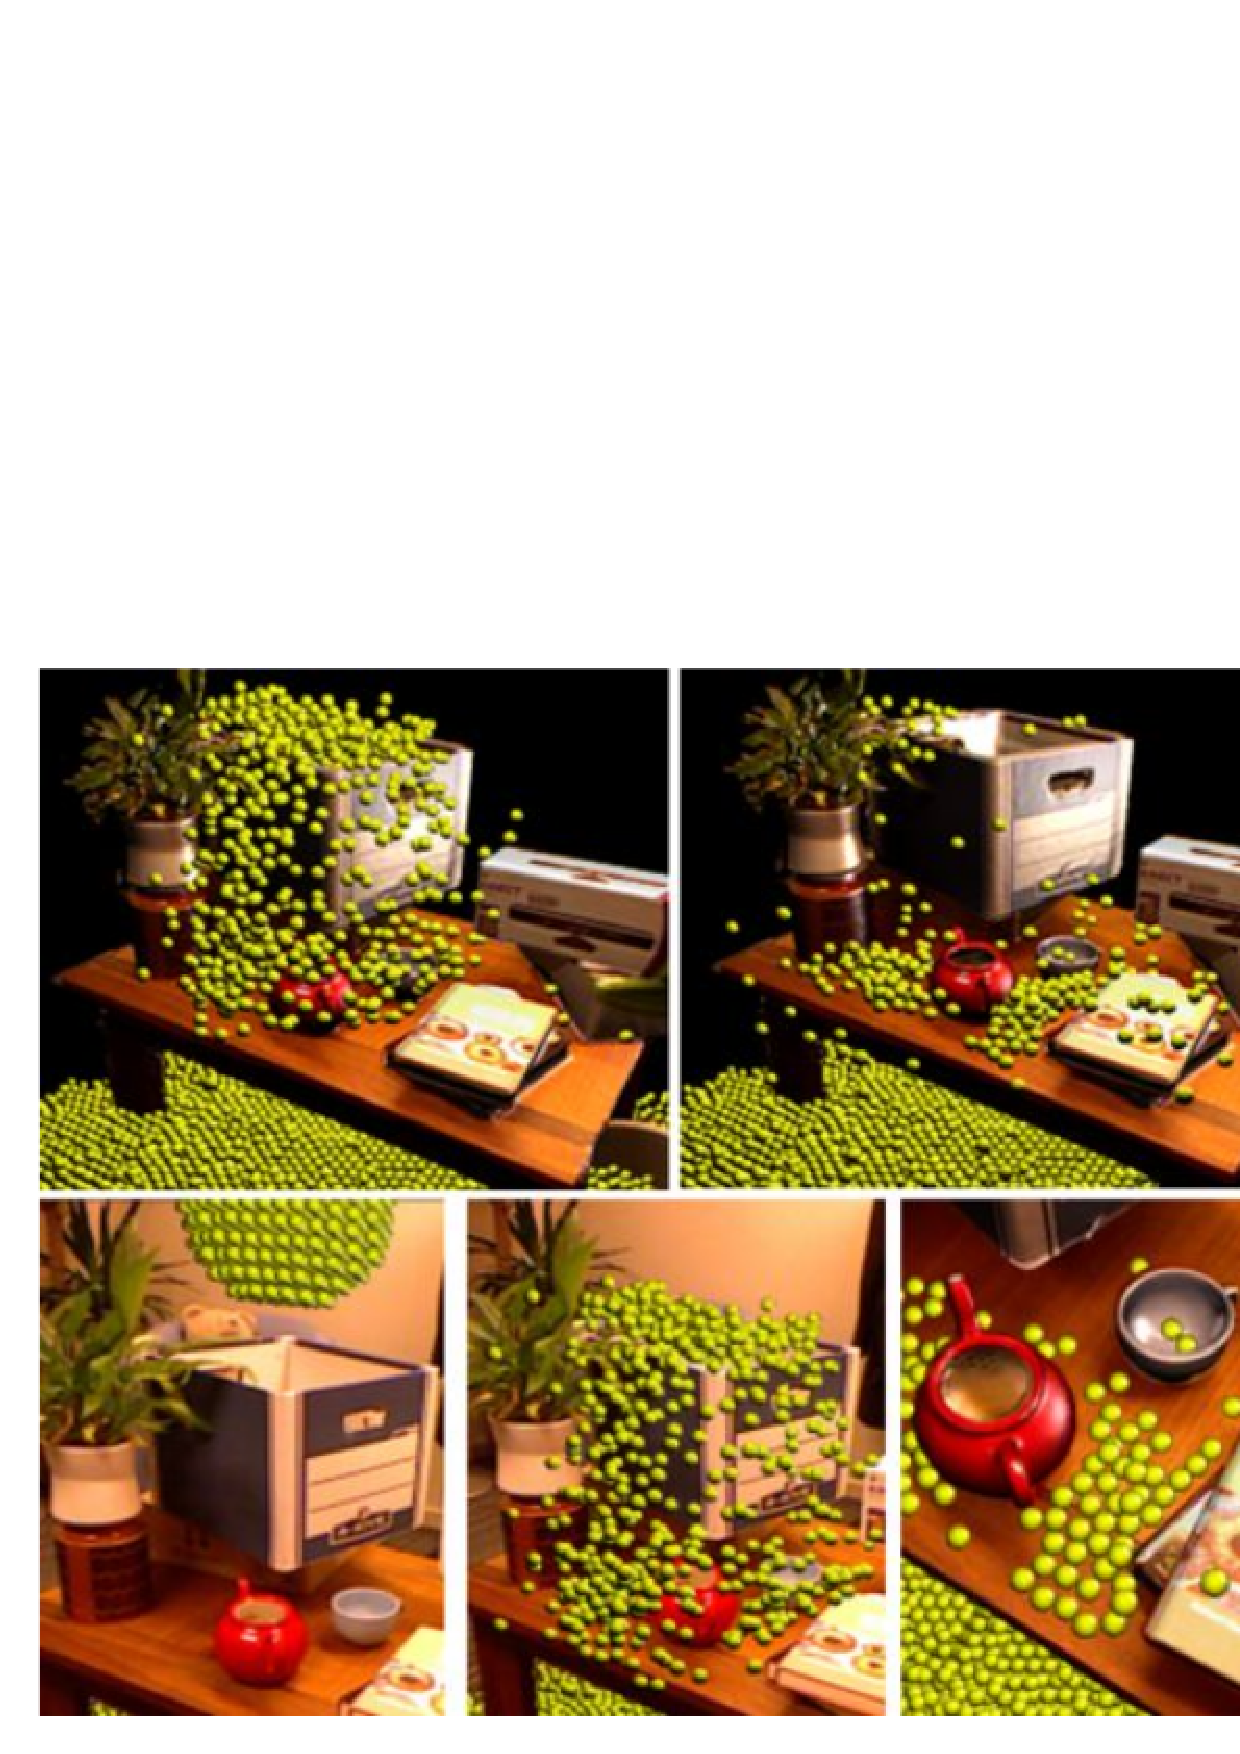
\includegraphics[scale=0.34]{images/izadi}
\caption{Reconstructed 3D scene with thousands of virtual particles}
\label{fig:izadi}
\end{center}
\end{figure}


All the 3D reconstruction methods can have problems with non lambertian 
surfaces and they need to make some assumptions about the surfaces reflectance. For example if we are using 
an infrared structured light pattern depth camera and the object that we are registering absorbs the infrared light, 
the reconstruction will fail. Similar problems can occur with laser scanners. 
Some materials such as glass or water can ruin the reconstruction.












\chapter{Sensor}
\index{Sensor}

\section{Pinhole Camera Model}

The pinhole camera model describes the mathematical relationship between the points of the image plane and the 3D points captured by an 
ideal pinhole camera. In the context of this work, this model is useful to explain how the depth is calculated by Kinect and 
how to reproject points in the photoconsistency method.

\begin{figure}[H]
\begin{center}
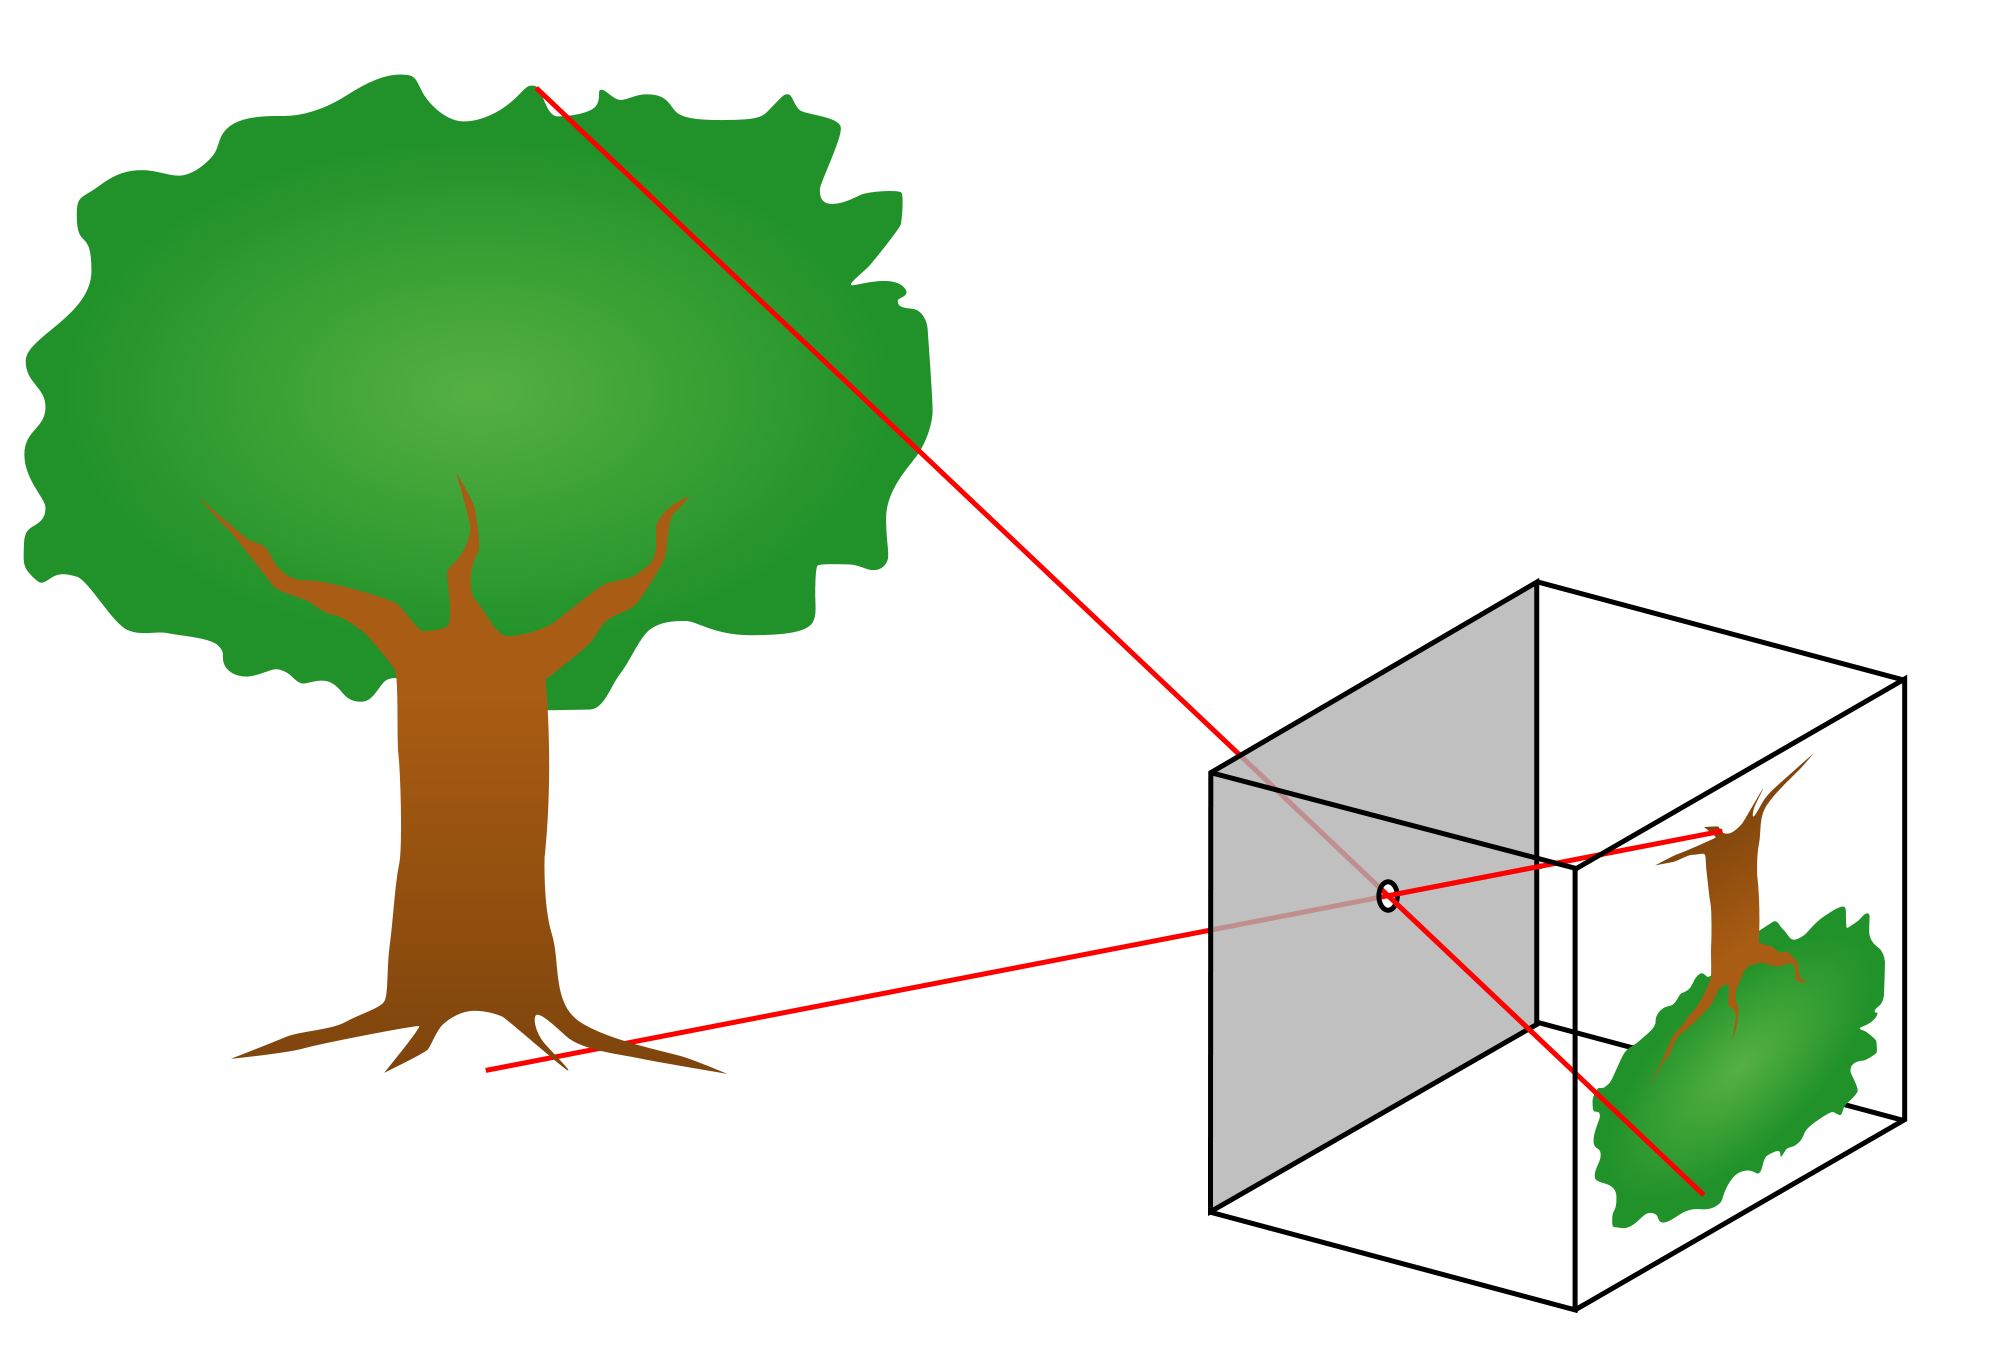
\includegraphics[scale=0.15]{images/pinhole-camera}
\caption{Pinhole camera}
\label{fig:pinhole}
\end{center}
\end{figure}

In the pinhole camera all rays pass from the scene to a photosensitive material through a pinhole, in order to form the image.

\begin{figure}[H]
\begin{center}
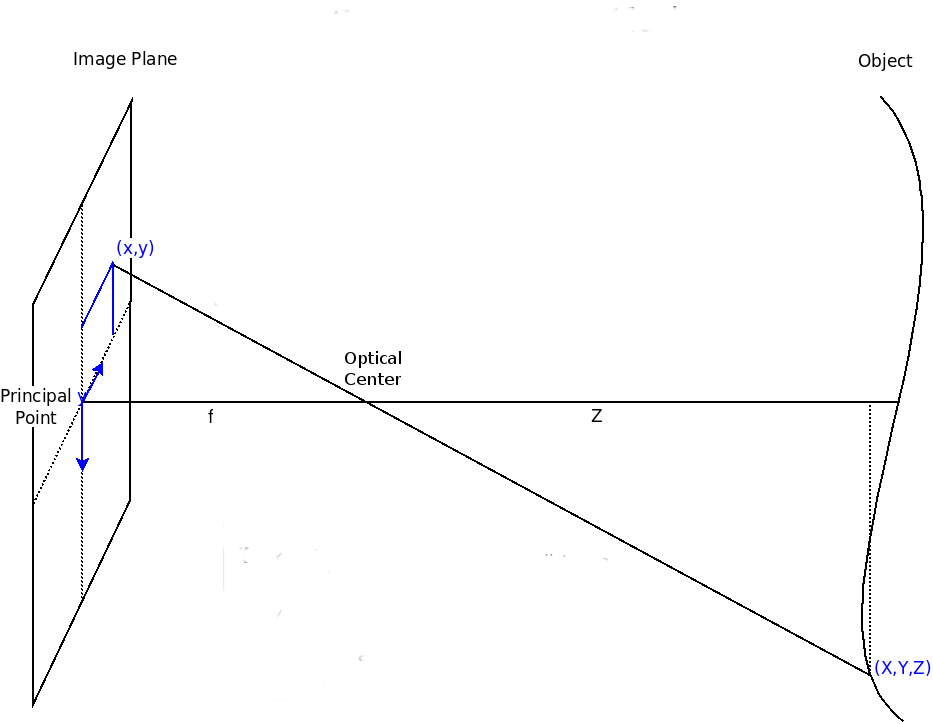
\includegraphics[scale=0.25]{images/pinhole-coordinates}
\caption{Pinhole camera coordinates system}
\label{fig:pinhole}
\end{center}
\end{figure}


The transformation between world coordinates point P(X,Y,Z) and image coordinates p(x,y) is described as 
follows:

\begin{equation}
\label{eq:disparity2}
 x = \frac{f*X}{Z}
\end{equation}

\begin{equation}
\label{eq:disparity2}
 y = \frac{f*Y}{Z}
\end{equation}

This equations are  obtained using triangles similarity.

\section{Sensor Depth Calculation}

The Kinect sensor consists of an infrared laser emitter, an 
infrared camera and an RGB camera. The laser source emits a single 
beam which is split into multiple beams by a diffraction 
grating to create a constant 
pattern of speckles projected onto the scene. This pattern is 
captured by the infrared camera and is correlated against a 
reference pattern. The reference pattern is obtained by capturing 
a plane at a known distance from the sensor, and is stored in the 
memory of the sensor. When a speckle is projected on an object 
whose distance to the sensor is smaller or larger than that of the 
reference plane the position of the speckle in the infrared image 
will be shifted in the direction of the baseline between the laser 
projector and the perspective centre of the infrared camera. 
These shifts are measured for all speckles by a simple image 
correlation procedure, which yields a disparity image \cite{khoshelham2011accuracy} . For each 
pixel the distance to the sensor can then be retrieved from the 
corresponding disparity.



\begin{figure}[h!]
\begin{center}
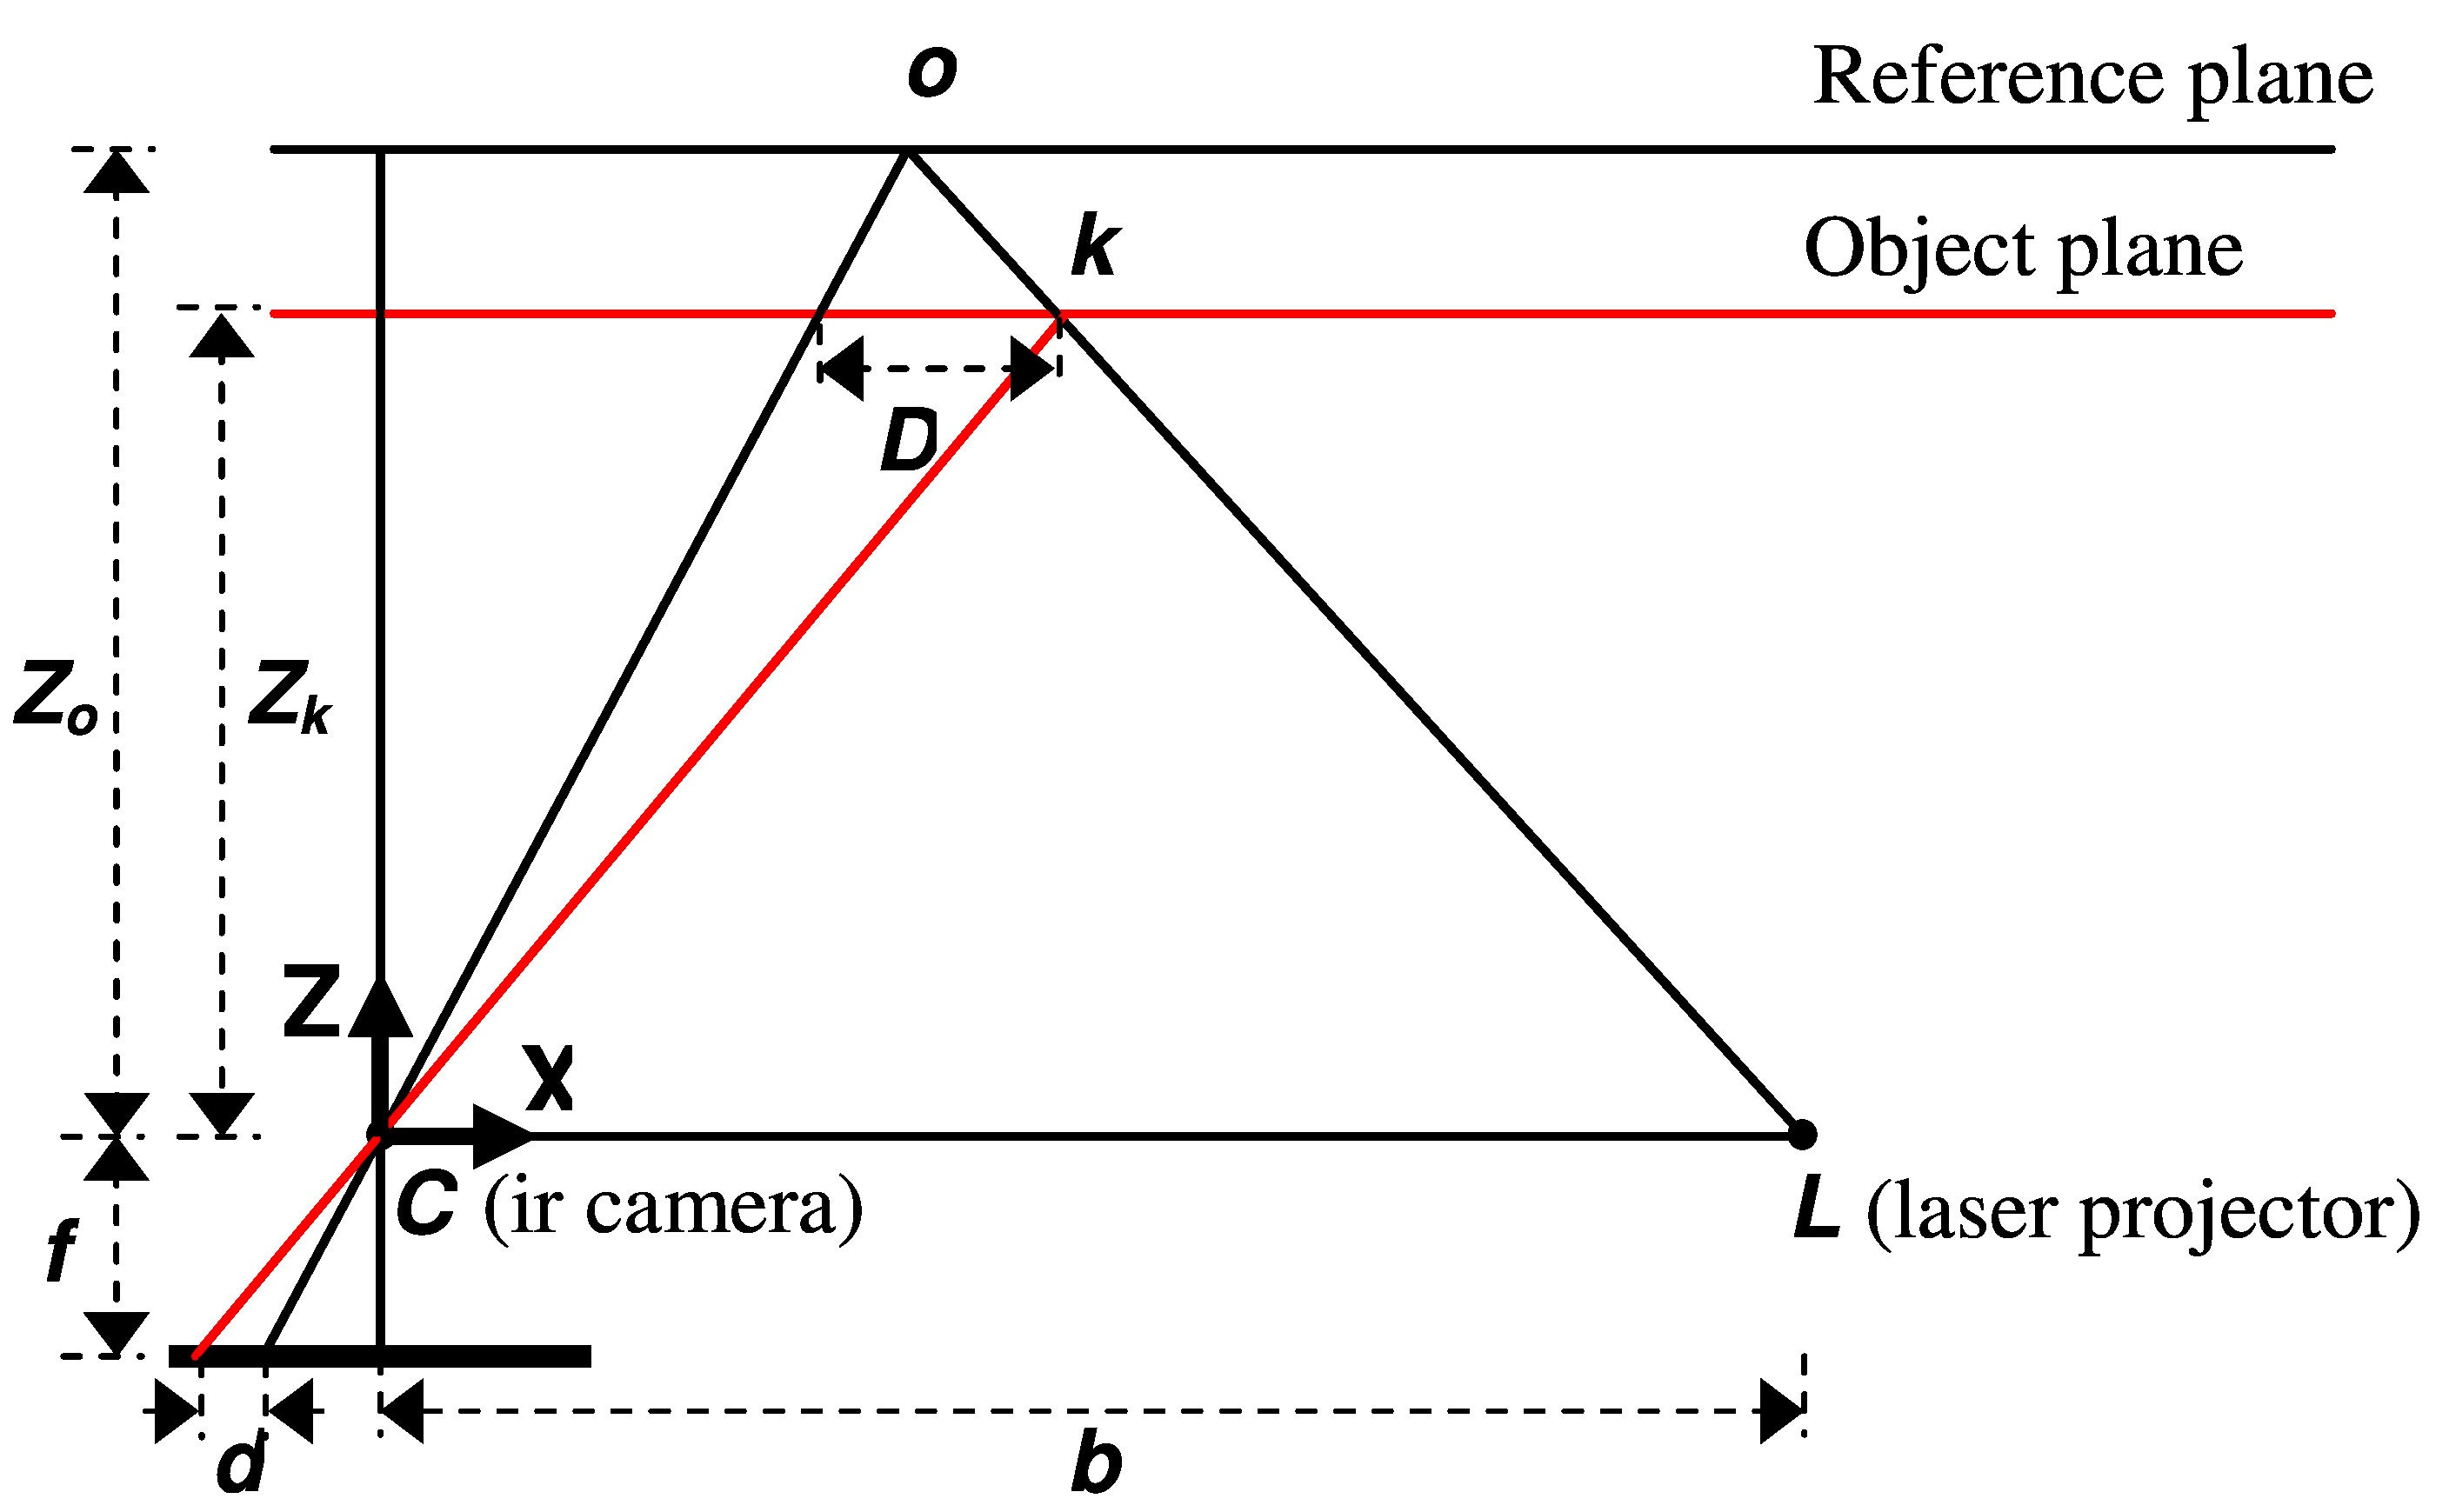
\includegraphics[scale=1]{images/kinect_triangulation}
\caption{Schematic representation of depth-disparity relation \cite{khoshelham2011accuracy}}
\label{fig:disparity}
\end{center}
\end{figure}

\begin{equation}
\label{eq:disparity1}
 \frac{D}{b} = \frac{Z_0 - Z_k}{Z_0} 
\end{equation}


\begin{equation}
\label{eq:disparity2}
 \frac{d}{f} = \frac{D}{Z_k} 
\end{equation}

Then $Z_k$ can be obtained from \ref{eq:disparity1} and \ref{eq:disparity2}. Where variables $Z_0$,$b$ and $f$ are known.

\section{Sensor Captured Data}

The sensor obtains two images: An RGB color image and a depth map.

The RGB color image has three channels: Red, Green and Blue. And each image color is generated 
combining this three colors. With a resolution of 640x480 pixels and 1 byte per channel. The sensor can 
capture color images at higher resolutions, but in our case we need just one color per depth map pixel.

The depth map is like a gray scale image where the value of each pixel is the object distance to the sensor in the viewing axis. 
The depth map is an image with a resolution of 640x480 and one channel of 2 bytes. We use meters as distance unit.

\begin{figure}[h!]
\begin{center}
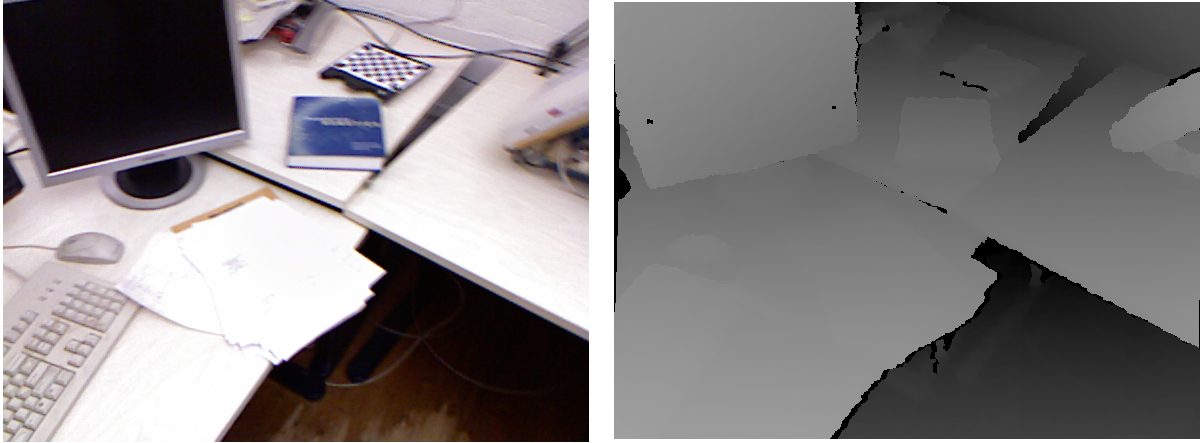
\includegraphics[scale=0.3]{images/color_depth.png}
\caption{Left: RGB image, right: depth map converted to a grayscale image (0-255 values) for visualization purposes}
\label{fig:colordepth}
\end{center}
\end{figure}


\begin{figure}[h!]
\begin{center}
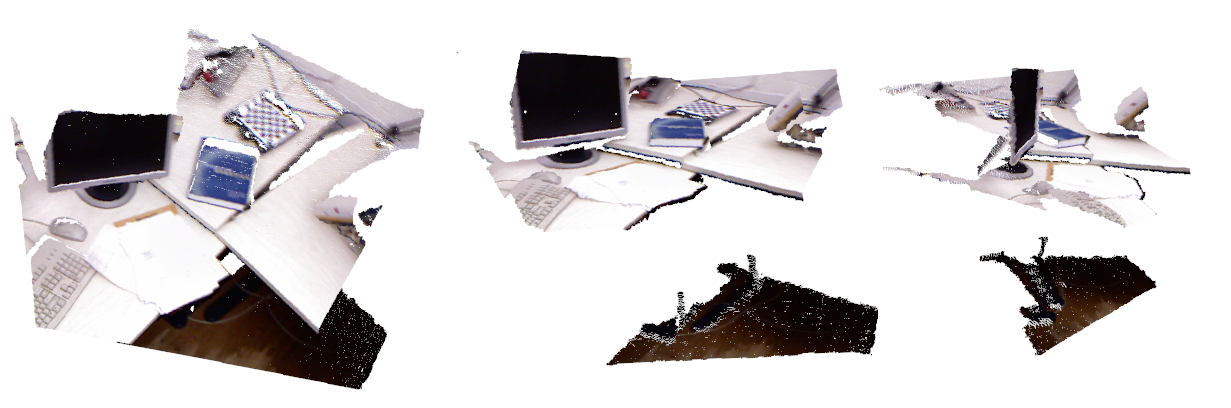
\includegraphics[scale=0.25]{images/3d_point_cloud.png}
\caption{Different perspectives of 3D color point cloud obtained combining the RGB image colors and the depth map 3D points}
\label{fig:colorpcloud}
\end{center}
\end{figure}


The depth map implicity contains the objects world coordinates, the relation between depth map 
and world coordinates is described as follows:

\begin{equation}
\label{eq:dasdf}
 X=\frac{(x-cx)*Z}{f}
\end{equation}

\begin{equation}
\label{eq:dispadsfy2}
 Y=\frac{(y-cy)*Z}{f}
\end{equation}


Where $(cx,cy)$ is the image principal point (projection of optical center on the image plane), f is the camera 
focal length, $(x,y)$ are the 2D coordinates in the depth map plane (640 pixels width, 480 pixels height) and $Z$ is the distance in the viewing axis from the camera to the object that is in position $(x,y)$ of depth map.

\begin{figure}[H]
\begin{center}
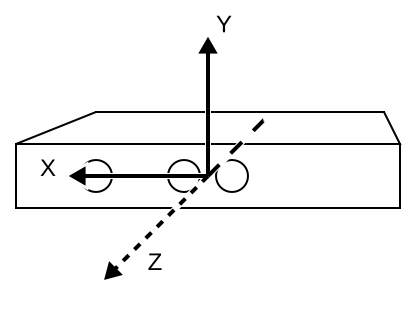
\includegraphics[scale=0.55]{images/coordinates}
\caption{Kinect coordinates system}
\label{fig:coordinates}
\end{center}
\end{figure}

In this work we will use the RGB image, the depth map and the point cloud obtained combining both.




\chapter{Proposal}
\index{Proposal}

The most used algorithm to register point clouds into a common coordinate 
system is called Iterative Closest Point (ICP) \cite{mckay92}. Given two point clouds, 
this algorithm finds the best rigid transformation to align both clouds. 

This algorithm has some drawbacks, such as being susceptible to local minimum, 
have small convergence basin, and in general needing a high number of iterations \cite{Rusu2009}. 
For this reason additional techniques are used in combination with ICP to compute a good approximation 
of the desired rigid transformation. Some of these techniques involve to filter the point clouds prior 
to apply the algorithm, look for a good initial estimation of the transformation to reduce algorithm 
iterations, applying some optimization techniques to improve the overall result, etc. 


This proposal combines ICP with filtering techniques in order to work with RGB-D data, combining the use of geometrical 
and visual clues in order to reduce the computational cost and improve the obtained results. Also, a pose graph optimization 
algorithm is applied, obtaining promising results.

\section{Bilateral Filter}


The depth maps captured by a low cost RGB-D camera usually contains noise, this can be 
consequence of materials reflectance, device imperfections, object fast movement, distance to the 
sensor, etc. 

In order to reduce the effect of noise, it is natural to use some kind of filter, as usual in computer 
vision, a typical filter will take information of a pixel and its neighborhood to generate a new image. 
If the image is smooth, without abrupt changes in intensity, a simple average could be enough. However, this 
is not the case in the presence of edges or corners, areas where the intensity changes sharply. 
The bilateral filter deals with this problem, giving to each neighbor a weight based on its closeness  
to the center pixel. In a grayscale image it takes into account 
the neighbor intensity distance and location distance (in image plane) to calculate the weight.  A depth map is very similar to a grayscale 
image, the only difference is that the depth map represents geometrical information (3D points) and usually contains holes 
(areas where the sensor failed to measure distance). 

A bilateral filter was applied to the depth maps, using the euclidean distance and the distance along the $z$ axis to calculate 
the weight of each pixel neighbor in the depth map. 

In a filter window centered at a 3D point $p$, corresponding to one depth map pixel, 
the weighted average was calculated using the following weight for each neighbor:


$$ w(p,q,\sigma_d,\sigma_z) = k(d(p,q),\sigma_d) k(z(p,q),\sigma_z)\ , $$

\noindent where 

$$ k(v,\sigma) = \frac{e^{-v^2}}{2*\sigma^2}\ , $$
$$ d(p,q) = ||p - q||\ , $$
$$ z(p,q) = |p_z - q_z|\ , $$
$$ p = (p_x,p_y,p_z)\ , $$ 
$$ q = (q_x,q_y,q_z)\ . $$

\noindent $p$ is the 3D coordinate of central point and $q$ the 3D coordinate of one of its neighbors. 3D coordinates are obtained using
 the depth map and equations (\ref{eq:depthmapx}) and (\ref{eq:depthmapy}).  Each point has a weight that depends on its euclidean distance and
 the distance along the $z$ axis, to the central point. The parameter $\sigma_d$ defines 
the neighborhood, all points of the depth map that are at euclidean distance $2*\sigma_d$ or less from the central point are considered, the 
central point itself also is considered as part of the neighborhood. Parameters $\sigma_d$ and $\sigma_z$ are obtained empirically.


Let 


$$ W = \sum\limits_{q\ \in\ p\ neighborhood} {w(p,q,\sigma_d,\sigma_z)}\ ,$$

\noindent the final value of the central pixel of the depth map that corresponds to the 3D point $(p_x,p_y,p_z)$ is then

$$p_z' = \frac{1}{W}\sum\limits_{q\ \in\ p\ neighborhood}{w(p,q,\sigma_d,\sigma_z)q_z}\ ,$$


After applying this filter we obtain a smoothed version of the depth map, without loosing edges and important geometrical information.
A detailed explanation of the bilateral filter can be found in \cite{TomasiBilateral}.


\section{Borders Filter}

Edges are widely used in computer vision, they contain rich information about texture 
and geometry, for this reason edges are features that are usefull for several tasks, 
such as object recognition, object traking, etc.


The Sobel filter is a wellknown edge detector. To apply this filter is necessary to 
convolve the image with two 3x3 matrices, to find intensity changes in vertical and 
horizontal directions:

\begin{center}
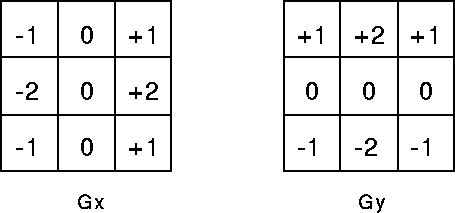
\includegraphics[scale=0.35]{images/sobel}
\end{center}

Then both results are merged using the bellow expression and a threshold is used to filter out non interest areas:

\begin{equation}
G = \sqrt{G_x^2+ G_y^2}
\label{eq:sobelGrad}
\end{equation}

This filter was used to obtain a representative set of points, avoiding that walls and another 
plain surfaces containing a huge amount of data, lead to an incorrect alineation.
There are more advanced edge filtering techniques, such as the Canny edge filter, but it involves 
a larger set of convolutions and operations. Since we don't need a high accuracy edge detection, the Sobel 
filter is enough to reduce the set of points used in the alineation process. 

The filter was applied directly into a grayscale representation of the original RGB image. Obtaining a binary image 
that contains edges representing geometrical and visual changes in the scene. 
This image can be used along with the depth map to reduce the point cloud size. Because dataset RGB and depth map images are 
calibrated, a pixel (x,y) in the RGB image corresponds to the same (x,y) location in the depth map. Thus, we can perform filtering 
in the RGB image and then modify depth map using the same coordinates. The binary image obtained from Sobel filter, was used 
to reject all points not corresponding
to these edges in the depth map. 

Edge filtering was applied
to the image instead of the depth map. Because using this approach it is possible to find corresponcendes between rich textured 
surfaces, even if they don't exhibit local geometrical changes.

The applied threshold for the Sobel filter was low, in order to have thicker edges. Because if too few points pass the filter, important information 
could be lost, difficulting a correct alieation


\begin{figure}
\begin{center}
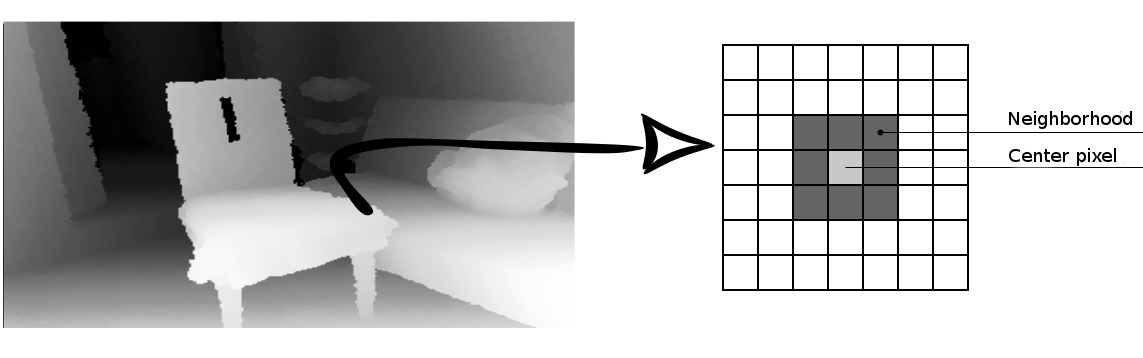
\includegraphics[scale=0.25]{images/vecindarioDepth}
\end{center}
\caption{Depth map pixel neighboorhod}
\label{fig:neighboor}
\end{figure}

In combination with a low threshold used in the Sobel filter applied to the grayscale image, all points of the neighborhood of the corresponding depth map pixels passing the Sobel filter were added. 
The neighborhood is defined as shown in figure ~\ref{fig:neighboor}. The purpose of this is to have enough points even if few points
 pass Sobel filter.

This filter is applied to both, source and target captures. Making this, it is possible to apply a very useful filtering: remove 
from both point clouds all the points that are not in common. For this, the rotation and translation 
of the source Sobel filtered 2D image that minimizes the distance between the closest pixels of the Sobel filtered target 2D image is found and 
then applied to each pixel of the source depth map, 
allowing perforing an AND operation as follows: if transformed source depth map pixel has a correspondent pixel in the target depth map and 
the euclidean distance (in the 3D space) is less than a threshold, maintain both pixels (of source and target depth maps), in other case reject them. 

 As result, we work with two point clouds that have a huge amount of overlaping points, improving the alineation 
result. The AND ensures that both depth map pixels (from source and target depth maps) are present in the two point clouds (at least from viewing 
perspective) and the distance filtering filters out pairs of points that pass the AND filter, but are too far in the euclidean space.

\begin{figure}[H]
\begin{center}
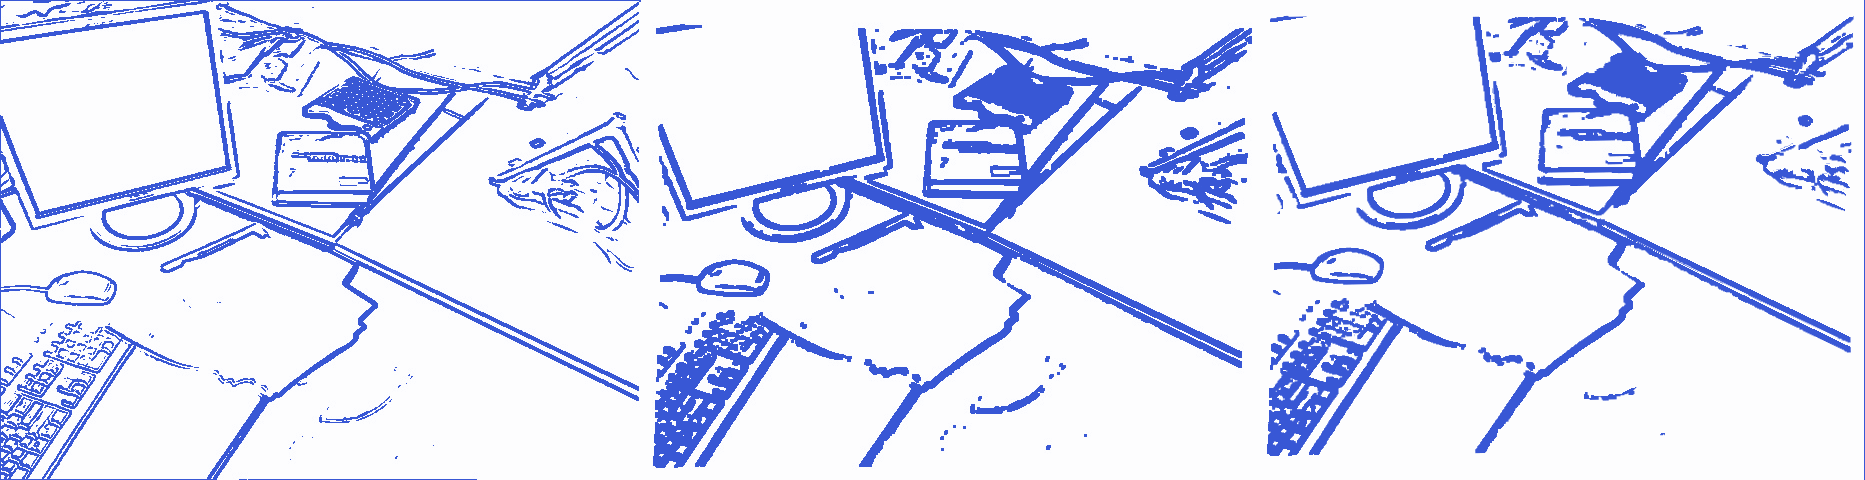
\includegraphics[scale=0.2]{images/borders_steps.png}
\caption{Left: Image after applying sobel filter, middle: Image after adding depth map neighborhood points, right: Image after
applying AND operation and distance filtering between the two consecutive point clouds}
\end{center}
\end{figure}


\begin{figure}[H]
\begin{center}
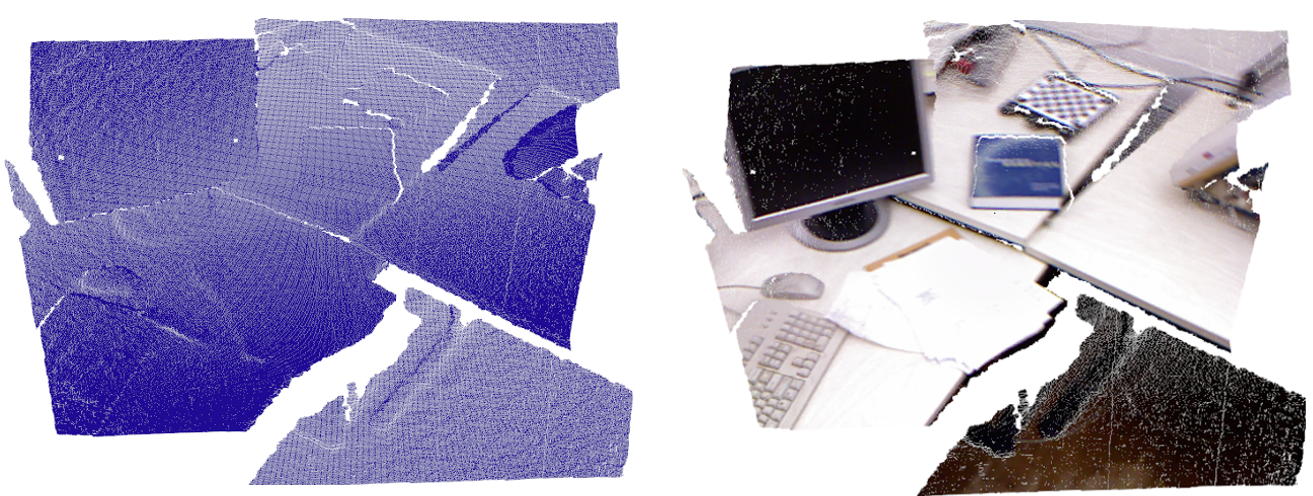
\includegraphics[scale=0.3]{images/borders_orig.png}
\caption{One of the point clouds before applying filter}
\end{center}
\end{figure}


\begin{figure}[H]
\begin{center}
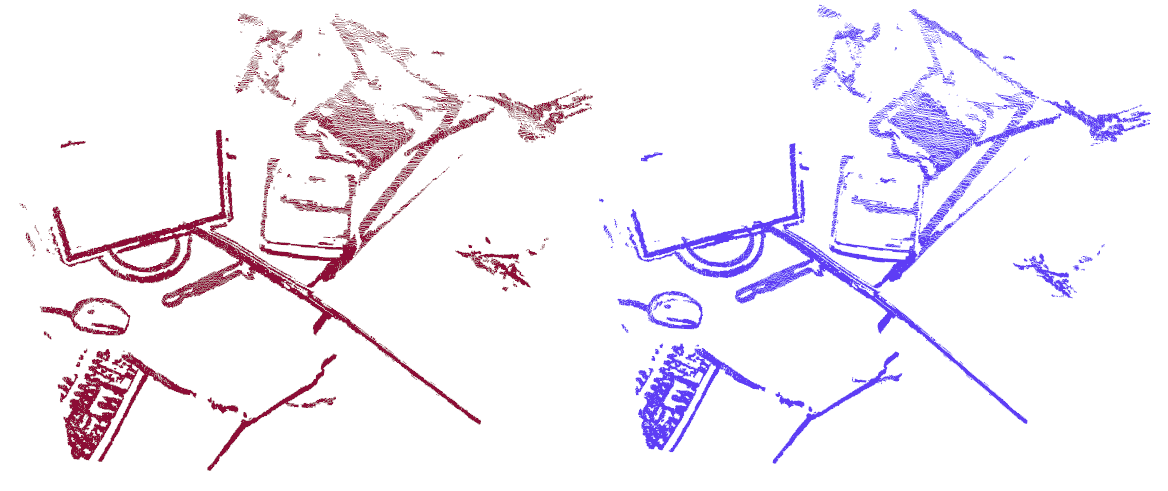
\includegraphics[scale=0.3]{images/borders_consec.png}
\caption{Two consecutive point clouds  after border filtering}
\end{center}
\end{figure}

\begin{figure}[H]
\begin{center}
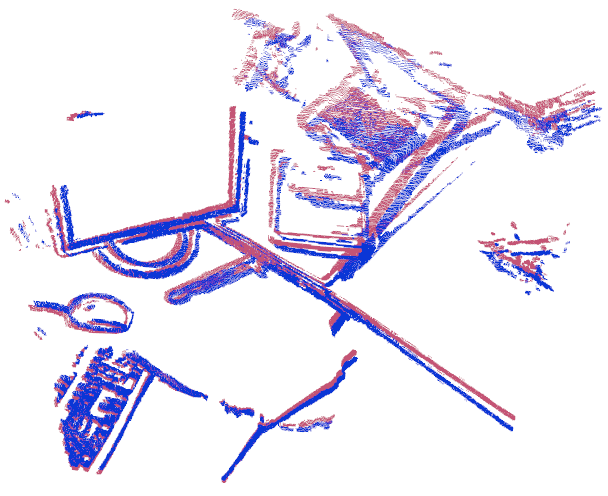
\includegraphics[scale=0.3]{images/borders_both.png}
\caption{Both filtered point clouds shown in the same coordinate system}
\end{center}
\end{figure}


\begin{algorithm}[H]
\caption{Edge filtering algorithm}
\begin{algorithmic}[1]
\State grayImageSrc = RGBtoGray(srcImage)
\State grayImageTgt = RGBtoGray(tgtImage)
\State sobelSrc = sobelFilter(grayImageSrc)
\State sobelTgt = sobelFilter(grayImageTgt)
\State T = FindRigidTransformation(sobelSrc,sobelTgt)
\ForAll {x in [0-640] and y in [0-320] } 
\If {$sobelSrc(x,y) > 0$ AND $DepthMapSrc(x,y) > 0$}
\State p = (x,y,DepthMapSrc(x,y))
\State (projx,projy) = applyRigidTransformation(T,x,y);
\If { $DepthMapTgt(projx,projy) > 0$}
\State pproj = (projx,projy,DepthMapTgt(projx,projy))
\If { $euclideanDist(p,pproj) < DMAX$}
\State srcPointCloud.addPoint(p)
\State tgtPointCloud.addPoint(pproj)
\EndIf
\EndIf
\EndIf
\EndFor
\end{algorithmic}
\end{algorithm}

Where sobelfilter is a threshold applied to image filtered with Sobel operators \ref{eq:sobelGrad}, T is a 3x3 rigid transformation matrix (2D rotation, 2D translation). DMAX is the maximum distance allowed between the source cloud point and corresponding target cloud point. 
Its value was setted in 0.1 (10 cm).  This value was determined empirically.

The key idea is that two consecutive images are almost identical, 
with different orientations because they where captured from different perspectives. This allows 
to filter from the two point clouds those points that have no match in the other point cloud.


 

\index{Image Correspondences}

\section{Image Correspondences}

\subsection{Corners}

There are several techniques to track an object. If there is information about the object of interest the problem 
can be simplified using this information to restrict the search space, for example to certain color or shape.
 By the other hand if the object to track is unknown, it is necessary to find a more general feature, that is 
more likely to be found on the unknown interest objects. The corners are good features for this purpose. A corner 
is a point on the image where there are gradient variations on two orthogonal directions.

The most common definition of a corner is gived by Harris corners method.

Consider a function E(u,v), to measure a difference between the pixels of a window (a region of the image) and 
a window shifted (u,v) units:

\begin{equation}
E(u,v) = \sum\limits_{x,y} { w(x,y) [I(x + u, y +v) - I(x,y)]^2  }\ .
\label{eq:harris1}
\end{equation}

We loop over a neighborhood defined by different values of (x,y) and calculate 
the difference of each pixel located at (x,y) with some other pixel located at (x+u,y+v). 
The function w(x,y) defines the window where we are working, in the case of a square windows, 
it has values 1 for pixels inside the window and 0 for other pixels. In the case of a circular 
window a Gaussian function can be used. 

E(u,v) will have bigger values when the window is centered in a corner. For this reason we want 
to detect when E(u,v) is maximum. With this purpose on mind, we can express $I(x + u, y +v)$ in a more convenient
 way using a Taylor expansion:

$$
I(x+u,y +v) = I(x,y) + I_xu + I_yv + Higher Order Terms \ ,
$$ 

\noindent where 

$$
I_x = \frac{\partial{I(x,y)}}{\partial{x}}\ ,
$$

$$
I_y = \frac{\partial{I(x,y)}}{\partial{y}}\ .
$$

Then we can use the following approximation:

$$
I(x+u,y +v) \approx I(x,y) + I_xu + I_yv\ ,
$$

$$
I(x+u,y +v) \approx I(x,y) + \begin{bmatrix} I_x & I_y \end{bmatrix} \begin{bmatrix} u \\ v \end{bmatrix}\ ,
$$ 

\noindent replacing this in \ref{eq:harris1} we get:

$$
E(u,v) \approx \sum\limits_{x,y} { w(x,y) [I(x,y)  + \begin{bmatrix} I_x & I_y \end{bmatrix} \begin{bmatrix} u \\ v \end{bmatrix} - I(x,y)]^2  }\ ,
$$

$$
E(u,v) \approx \sum\limits_{x,y} { w(x,y) [\begin{bmatrix} I_x & I_y \end{bmatrix} \begin{bmatrix} u \\ v \end{bmatrix} ]^2  }\ ,
$$

$$
E(u,v) \approx \begin{bmatrix} u & v \end{bmatrix} \sum\limits_{x,y} w(x,y) \underbrace{\begin{bmatrix} {I_x}^2 & I_x I_y \\ I_x I_y & {I_y}^2 \end{bmatrix}}_{H} \begin{bmatrix} u \\ v \end{bmatrix}\ .
$$


Eigenvalues of H can be used to detect corners. When both eigenvalues have large magnitude, the window contains a corner. If just one 
eigenvalue has large magnitude we have an edge and if both eigenvalues have small magnitude we have a plain surface.

Once we have corners, we can find the movement of each corner between two successive images using Optical Flow. The objective 
is to find correspondences (common points) between the two images.

\subsection{Optical Flow}

The optical flow methods are used to calculate motion between two successive image captures which are taken
 at two different times: $t$ and $t + \Delta t$.

These methods have two main assumptions about the frames \cite{sonka2007}:

\begin{enumerate}
\item The observed brightness of any object point is constant over time.
\item Nearby points in the image plane move in a similar manner (velocity smoothness).
\end{enumerate}

\begin{figure}[h!]
\begin{center}
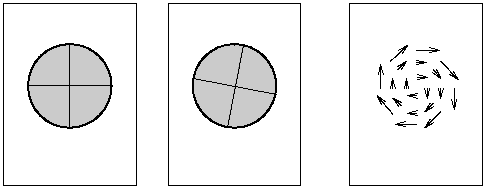
\includegraphics[scale=0.6]{images/oflow}
\caption{Image at time $t$, image at time $t + \Delta t$ and optical flow.}
\label{fig:oflow}
\end{center}
\end{figure}

There are two kinds of optical flow: dense and sparse. Dense optical flow means to calculate a direction vector for each pixel of the image and sparse optical flow is calculate direction vector just for those pixels of the image 
who satisfy certain conditions.

Dense optical flow is computationally expensive and it is difficult to find the direction vector 
for plain color areas. For example in an image of a white paper or a wall
there are a lot of pixels with the same properties and it is necessary to perform some kind of interpolation to give a direction vector
 to each one of these pixels. 
By the other hand, sparse optical flow just consider pixels with more odds of matching between the two frames.

\subsection{Lukas-Kanade Method}
\label{sec:oflow}

The Lukas-Kanade method is a sparse optical flow method, that 
uses a search window for each pixel of interest and assume that all the pixels 
inside the search window have the same direction vector.


We have two images: $I(x,y,t)$ and $I(x,y,t+\Delta t)$.
If optical flow conditions are meet :

\begin{equation}
\label{eq:oflowrel}
I(x + \Delta x,y + \Delta y, t + \Delta t) = I(x,y,t)\ .
\end{equation}

We can express $I(x + \Delta x, y + \Delta y, t + \Delta t)$ using Taylor series as:

\begin{equation}
\label{eq:oflowtaylor}
I(x + \Delta x, y + \Delta y, t + \Delta t) = I(x,y,t) + \frac{\partial I}{\partial y} \Delta y + \
 \frac{\partial I}{\partial x} \Delta x  + \frac{\partial I}{\partial t} \Delta t + Higher Order Terms \ .
\end{equation}

If we combine \ref{eq:oflowrel} and \ref{eq:oflowtaylor} we obtain the general optical flow equation :


$$ I(x,y,t) + \frac{\partial I}{\partial y} \Delta y + \
 \frac{\partial I}{\partial x} \Delta x  + \frac{\partial I}{\partial t} \Delta t + Higher Order Terms = I(x,y,t)\ , $$


$$ \frac{\partial I}{\partial y} \Delta y + \
 \frac{\partial I}{\partial x} \Delta x  + \frac{\partial I}{\partial t} \Delta t \approx 0 \hspace{0.5cm} \backslash \cdot \frac{1}{\Delta t}\ ,  $$


$$ \frac{\partial I}{\partial y} \frac{\Delta y}{\Delta t} + \
 \frac{\partial I}{\partial x} \frac{\Delta x}{\Delta t}  + \frac{\partial I}{\partial t}  \approx 0 \ , $$


\noindent let :

$$ V_x = \frac{\Delta x}{\Delta t}\ , $$
$$ V_y = \frac{\Delta y}{\Delta t}\ , $$
$$ I_x = \frac{\partial I}{\partial x}\ ,$$
$$ I_y = \frac{\partial I}{\partial y}\ ,$$

\noindent and finally we get :

$$ I_x V_x + I_y V_y = -I_t \ ,$$

\begin{equation}
\label{eq:oflowgeneral}
\nabla{\vec{I}} \cdot \vec{V} = -I_t \ .
\end{equation}

We have an equation with two unknowns $V_x$ and $V_y$, we can't solve it without additional restrictions.

The Lukas-Kanade method assumes that all the pixels inside a window satisfy this equation for the same 
values of $V_x$ and $V_y$. Thus, if we have a $5\times5$ window, we have 25 equations with two unknowns :

$$
\begin{bmatrix}
I_x(p1) & I_y(p1) \\
I_x(p2) & I_y(p2) \\
... & ... \\
I_x(p25) & I_y(p25)\\
\end{bmatrix}  \ ,
\begin{bmatrix}
V_x \\
V_y\\
\end{bmatrix}
=
-\begin{bmatrix}
I_t(p1) \\
I_t(p2) \\
...     \\
I_t(p25) 
\end{bmatrix} \ ,
$$

where $p_1, p_2, ..., p_{25}$ are pixel 1, pixel 2, etc.

Let 

$$
A = 
\begin{bmatrix}
I_x(p1) & I_y(p1) \\
I_x(p2) & I_y(p2) \\
... & ... \\
I_x(p25) & I_y(p25)\\
\end{bmatrix}  \ ,
$$

$$
x=
\begin{bmatrix}
V_x \\
V_y\\
\end{bmatrix} \ ,
$$

$$
b=
-\begin{bmatrix}
I_t(p1) \\
I_t(p2) \\
...     \\
I_t(p25) 
\end{bmatrix} \ .
$$

\noindent Then we have the classical problem :

$$ 
Ax = b\ .
$$

\noindent A solution can be obtained by the least squares, using partial derivatives of the unknowns and equating to zero, the following expression
 is obtained:

$$
x = (A^T A)^{-1} A^T b \ .
$$


\noindent $A^T A$ will be invertible depending on the pixels of the image. Even if $A^T A $ is invertible, 
if its values are very small it can be ill conditioned. For this reason it is necessary to check the eigenvalues of $A^T A$, if they are zero or very small, then it is not possible to find a solution.

In order to increment the odds of obtaining a solution the Lukas Kanade method works only in the corners detected on the image, because corners are better points to be tracked.

\subsection{Speeded Up Robust Features}
\label{sec:surf}

The Speeded Up Robust Features (SURF) algorithm finds image features looking for strong responses in two orthogonal directions, in order to detect points that are strong to rotation and translation transformations. For this purpose the determinant of the Hessian matrix calculated for each pixel is used:


$$
H = \begin{bmatrix} I_{xx} & I_x I_y \\ I_x I_y & I_{yy} \end{bmatrix} \begin{bmatrix} u \\ v \end{bmatrix} \ ,
$$

$$
det(H) = I_{xx} I_{yy} - I_{xy}^2\ .
$$


\noindent The second order partial derivatives are approximated using just a box filter, in other words 
summing and subtracting pixel values instead of using the classical Gaussian weighing. 

\begin{figure}[!h]
\begin{center}
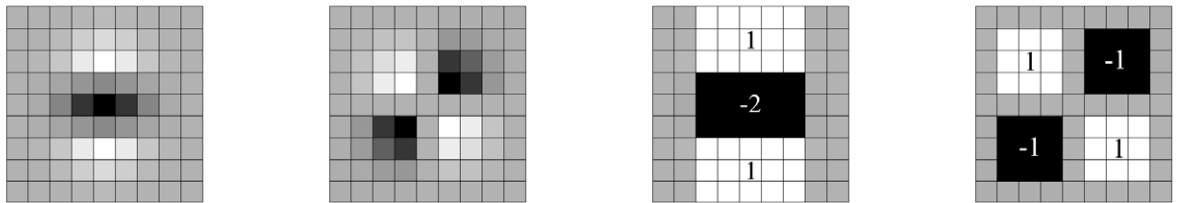
\includegraphics[scale=0.35]{images/surf_mask}
\caption{Left to right: the discretized and cropped Gaussian second order partial derivatives 
in y-direction and xy-direction, and approximations using box filters. 
Grey regions are equal to zero. Image extracted from \cite{Bay06surf}.}
\end{center}
\end{figure}

This filter is applied to each pixel of the image, obtaining the value $det(H)$ for each one of the pixels. 

When it is necessary to extract features from an image, the image  usually is scaled to different sizes (scale-space) in order 
to find image structures 
at different scales. SURF algorithm instead of scale the image, scales the filter applied to the 
image, increasing the speed of the calculations in one order of magnitude.

\begin{figure}[!h]
\begin{center}
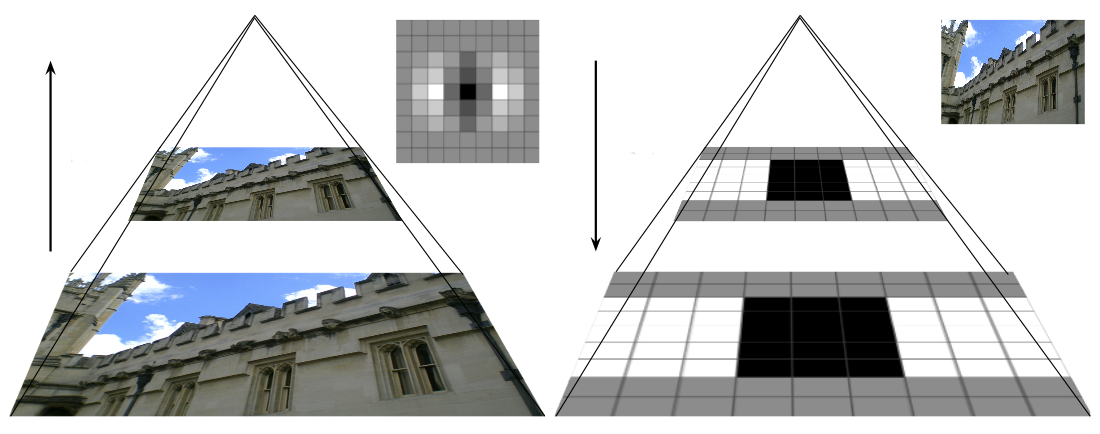
\includegraphics[scale=0.35]{images/surf_scale}
\caption{Left to right: traditional approach to produce scale-space, scaling image and applying Gaussian filter. SURF approach to produce scale-space, scaling the filter and maintaining the image size. Image extracted from \cite{miguel}.}
\end{center}
\end{figure}


In order to find interest points a non-maximal suppression is applied, in order to maintain only points above certain threshold. 

\begin{figure}[H]
\begin{center}
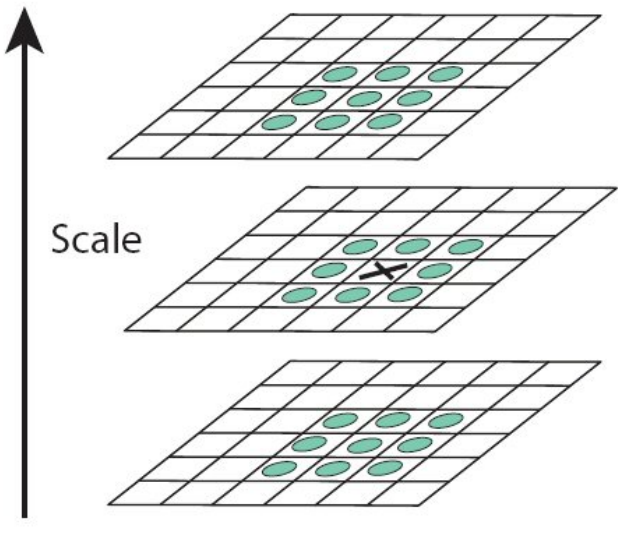
\includegraphics[scale=0.28]{images/surf_nb}
\caption{Non-Maximal Suppression. The pixel marked X is selected as a maximum if it is greater than the 
surrounding pixels on its interval and intervals above and below. Image extracted from \cite{OpenSURF}.}
\end{center}
\end{figure}

At the end of this step a set of interest points is obtained. Then an interpolation is applied, in order to find the location 
at sub-pixel accuracy.

Once the set of points is calculated, a descriptor to each point is generated. The descriptor is calculated relative to a dominant 
orientation, in order to reach rotation invariance.
 
The following features are used to describe a point $v=\{dx,dy,|dx|.|dy|\}$ this features are calculated in several regions 
around the interest point. Obtaining a vector of 64 components that is normalized to reduce the effect of changes in the image 
intensities. A complete explanation of how this algorithm works can be found in \cite{OpenSURF}



\section{Photoconsistency}

Having a estimation of rotation R and translation t, it is possible to reproject the 3D points to the 2D image plane using the 
camera parameters. If we have a point $p=(X,Y,Z)$ we can project it to the image plane using the following formula obtained 
from the pinhole camera model:

\begin{equation}
U(p) = (\frac{fX}{Z} - c_x, \frac{fY}{Z} - cy)
\label{eq:reproject}
\end{equation}

Where $f$ and $(cx,cy)$ denote the focal length and optical center of the pinhole camera model. 
We can apply the transformation R,t to the point before projecting it:

\begin{equation}
T(R,t,p) = Rp + t = p'
\end{equation}

Image coordinates  $p'$ are used to obtain image color in the target image, making a reprojection of $p'$ to the image plane.

Then we can apply the following error formula, that represents the color differences between the reprojected image and 
the target image. 

\begin{equation}
E(R,t) = \frac{1}{N} \sum\limits_{p \in pointCloudSource} |RGBsource(U(p)) - RGBtarget(U(p'))|
\end{equation}


Where:
\begin{itemize}
\item N is the number of points.
\item $U(p)$ is the reprojection function \ref{eq:reproject} that returns (x,y) image coordinates of an (X,Y,Z) point.
\item  $RGBsource(x,y)$ is function that returns a vector (R,G,B) representing image color at location (x,y). Where 
R,G,B are positive integers between 0 and 255. The same holds for $RGBtarget(x,y)$. Both functions represent 
source and target images respectively.
\end{itemize}

In this case the average color difference vector norm is used, but there are many ways of measure photoconsistency, 
for example using a color space different from RGB or using another error metric. Photoconsistency is widely used in 3D reconstuction, for example some works using it are \cite{Whelan13},\cite{kerl13icra} and \cite{Newcombe10livedense}



\section{Iterative Closest Point}

The ICP algorithm \cite{mckay92} is widely used for 3D reconstruction. This algorithm tries to find 
the optimal rotation and translation between two point clouds that minimizes the distance between corresponding 
points. Corresponding points are determined assigning to each point of one cloud, the closest point in the other cloud.

As result at each iteration we have a set of pairs of the closest points, where each pair contains one point of each cloud. This set 
of pairs changes from iteration to iteration, since the rotation and translation updates the points of one of the point clouds. If enough correct 
corresponding points are found in each iteration, the algorithm converges to the correct transformation that aligns both point clouds.


\begin{itemize}
\item $R$ : $3\times3$ Rotation matrix
\item $t$ : $3\times1$ Translation vector
\item $srcPointCloud,srcPointCloud',tgtPointCloud$ : Point sets $\in R^3$
\item $pointPairs$ : Pair set
\end{itemize}
%\small
\begin{algorithm}
\caption{ICP algorithm}
\begin{algorithmic}[1]
\State init(R,t)
\State srcPointCloud' $\leftarrow$ transform(srcPointCloud,R,t) 
\State pointPairs $\leftarrow$ closestPoints(srcPointCloud',tgtPointCloud)
\State $\{R,t\} \gets$ updateTransformation(pointPairs)
\State $e_i = meanSquareError(p)$
\If {$e_i < threshold$ OR  $i > maxIteracions$} 
	\State return R,t
\Else
	\State go to step 2
\EndIf
\end{algorithmic}
\end{algorithm}


We want to find R and t that minimizes the following expression:

$$ \sum\limits_{i=1}^n ||R a_i -  b_i - t ||^2 \ ,$$

\noindent where each $a_i,b_i$ is a vector $\in \mathbb{R}^3$, R is a $3\times3$ rotation matrix and t is a vector $\in \mathbb{R}^3$


We make a change of coordinates, placing the centroid of each cloud as origin:



\begin{align*}
 \bar{a} = \frac{1}{n} \sum\limits_{i=1}^n {a_i} \ ,\\ 
  \bar{b} = \frac{1}{n} \sum\limits_{i=1}^n {b_i} \ , \\  
   {a'}_i = a_i - \bar{a} \ , \\
   {b'}_i = b_i - \bar{b} \ ,
\end{align*}

\noindent replacing:

\[ \sum\limits_{i=1}^n ||R a_i -  b_i - t ||^2 = \sum\limits_{i=1}^n ||R ( {a'}_i + \bar{a} ) -  ( {b'}_i  + \bar{b} ) - t ||^2  \ . \] 

\noindent The desired translation is $t = R \bar{a} - \bar{b} $. We must consider the rotation in this expression, since 
the rotation of a point cloud will change the position of all points and as consequence the translation.

Replacing $t$ in our previous expression we get:
\begin{flalign*}
&\sum\limits_{i=1}^n ||R a'_i - b'_i ||^2  \ , \\ 
&=\sum\limits_{i=1}^n (R a'_i - b'_i)^t (R a'_i - b'_i) \ , \\
&=\sum\limits_{i=1}^n ( (R a'_i)^t R a'_i - (R a'_i)^t b'_i  - b_i^{\prime t} R a'_i + b_i^{\prime t} b'_i) \ , \\
&=\sum\limits_{i=1}^n ( a_i^{\prime t} R^t R a'_i - 2 b_i^{\prime t} R a'_i + b_i^{\prime t} b'_i) \ , \\ 
&=\sum\limits_{i=1}^n (a_i^{\prime t} a'_i -  2 b_i^{\prime t} R a'_i + b_i^{\prime t} b'_i) \ .
\end{flalign*}


\noindent Minimize the previous expression is equivalent to maximize:

\begin{align*}
& \sum\limits_{i=1}^n b_i^{\prime t} R a'_i =  Trace ( \sum\limits_{i=1}^n R a'_i  b_i^{\prime t} ) = Trace (RH) \ ,\\
& H=\sum\limits_{i=1}^n a'_i  b_i^{\prime t} \ . 
\end{align*}


Lemma (\ref{ap:lemma}): For any positive definite matrix $A A^t$ and any orthogonal matrix B

\[ Trace( A A^t ) \geq Trace (B A A^t) \ . \]


\noindent Now using this lemma we will maximize our expression:


Let's apply the SVD factorization to H, then:

\[ H = U \Sigma V^t \ , \]

\noindent where U and V are $3\times3$ orthonormal matrices and $\Sigma$ is a diagonal matrix with no negative elements.

Let $ R = V U^t $ then :

\begin{align*}
RH = VU^t U \Sigma V^t = V \Sigma V^t = V \Sigma^{\frac{1}{2}} (V \Sigma^{\frac{1}{2}})^t \ ,
\end{align*}

\noindent which is symmetrical and positive definite.
Therefore, from lemma, for any $3\times3$ orthonormal matrix B :

\[ Trace( R H ) \geq Trace( B R H ) \ . \]

Thus, the solution for our problem is :

\begin{align*}
R = V U^t \ , \\
t = R \bar{a} - \bar{b} \ .
\end{align*}


\noindent This means that if we apply the rotation $R$ and the translation $t$, to each point of the point cloud A, the distance between the
 closest points of 
transformed point cloud A with point cloud B will be minimal, when registering a set of points from a real 3D scene it allows aligning 
successive scene frames.

\section{Pose Graph Optimization}
\label{sec:posegraph}
When the amount of registered frames increments, the accumulated error 
becomes visible. There is a drift respect to the real sensor trajectory. 
In order to deal with this problem, the most common approach is to use a pose graph 
optimization algorithm. 


Each pose of the sensor (rotation and translation) represents a node of the 
graph and each restriction between two poses represents an edge. The relative 
transformation between two poses is used as restriction.


The first pose of the graph can be arbitrary, in our case is set as the identity. Subsequent 
poses are determined by using relative transformations between pairs of frames, applying 
proposed technique. Each sensor frame corresponds to a graph pose. 

We have a non-linear least squares minimization problem that can be described by the following equation:

$$ F(x) = \sum\limits_{<i,j> \in C } e(x_i,x_j,z_{ij})^T \Omega_{ij} e(x_i,x_j,z_{ij}) $$

$$ x^* = \mathop{\rm argmin}_x F(x) \ ,$$

\noindent where $x=\{x_1,x_2,...,x_n\}$ and each $x_i$ represents a parameter block , $z_{i,j}$ and $\Omega_{ij}$ represents the mean  
 and the information matrix  of a constraint 
relating parameters $x_i$ and $x_j$. In our case $x_i$ corresponds to a sensor pose, $z_{ij}$ is the 
relative transformation between $i$-$esim$ and $j$-$esim$ sensor frame, it is not affected by the accumulated error 
because it is a direct measure between the two frames and $\Omega_{ij}$ is the weight or 
the confidence we give to the restriction. $\Omega_{ij}$ is a $7\times7$ diagonal matrix, containing on its diagonal the confidence ($\in [0,1]$) for each 
parameter of the transformation. 

Poses and relative transformations are represented by a $7\times1$ vector containing a translation vector
 and a normalized quaternion for the rotation:

$$ \begin{bmatrix} tx & ty & tz & qx & qy & qz & qw \end{bmatrix} ^T \ .$$



Then $e_{ij}$ is an error vector ($7\times1$) defined as follows:

$$
e(x_i,x_j,z_{ij}) = z_{ij} - \hat{z_{ij}} \ ,
$$

\noindent where $\hat{z_{ij}}$ is the relative transformation between $x_i$ and $x_j$ obtained directly from the pose graph, for this reason 
it is affected by the accumulated error.

We want to find a graph configuration (updating the poses $x=\{x_1,x_2,...,x_n\}$), that reduces global error,
 correcting some poses in order to satisfy the restrictions.

This  non-linear least squares problem can be solved using 
methods such as for example Gauss-Newton or Levenberg-Marquard \cite{numericalOptBook}.

\begin{figure}[!h]
\begin{center}
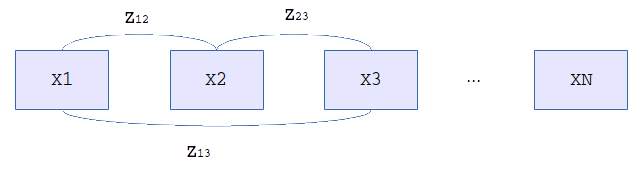
\includegraphics[scale=1.5]{images/graph_diagram2}
\caption{Graph of poses $(x_1,x_2,..)$ with constraints $(z_{12},z_{23},...)$ relating poses.}
\end{center}
\end{figure}

To simplify notation let: 

$$
e(x_i,x_j,z_{ij}) = e(x_i,x_j) = e_{ij}(x) \ ,
$$

\noindent we can approximate the previous function around one point:

\begin{equation}
\label{eq:errorAprox}
e_{ij}(x + \Delta x) \simeq e_{ij}(x) + J_{ij} \Delta x \ ,
\end{equation}

\noindent $J_{ij}$ is the Jacobian of the function evaluated in x. 


\begin{equation}
\label{eq:globalFunc}
F_{ij}(x + \Delta x) = e_{ij}(x + \Delta x)^T \Omega_{ij}  e_{ij}(x + \Delta x) \ .
\end{equation}

\noindent Replacing \ref{eq:errorAprox} in the global function:

\begin{equation}
\label{eq:globalFuncAprox}
F_{ij}(x + \Delta x) \simeq (e_{ij}(x) + J_{ij} \Delta x)^T \Omega_{ij}  (e_{ij}(x) + J_{ij} \Delta x) \ ,
\end{equation}

\begin{equation}
\label{eq:globalFuncAprox2}
 =  \underbrace{e_{ij}(x)^T \Omega_{ij} e_{ij}(x)}_{c_{ij}} + 2  \underbrace{e_{ij}(x)^T \Omega_{ij} J_{ij}}_{b_{ij}} \Delta x + \Delta x^T \underbrace{ J_{ij}^T  \Omega_{ij} J_{ij}}_{H_{ij}} \Delta x \ ,
\end{equation}

\begin{equation}
\label{eq:globalFuncAprox2}
 = c_{ij} + 2 b_{ij} \Delta x + \Delta x^T H_{ij} \Delta x \ ,
\end{equation}


\begin{equation}
F(x + \Delta x) =  \sum\limits_{<i,j> \in C } F_{ij}(x + \Delta x) \ ,
\end{equation}



\begin{equation}
\simeq  \sum\limits_{<i,j> \in C } c_{ij} + 2 b_{ij} \Delta x + \Delta x^T H_{ij} \Delta x \ ,
\end{equation}

\begin{equation}
\label{eq:lzn}
=   c + 2 b \Delta x + \Delta x^T H \Delta x \ ,
\end{equation}

\noindent where $c=\sum{c_{ij}}, b=\sum{b_{ij}}$ and $H=\sum{H_{ij}}$.

\noindent Then we want to know $\Delta x^*$, this is the correction to the nodes of the graph in order 
to have a minimum error. It can be obtained by solving the following linear system:

\begin{equation}
H \Delta x^* = -b \ .
\end{equation}

\noindent Having $\Delta x^*$ we can update the graph nodes:

\begin{equation}
x^* = x + \Delta x^* \ .
\end{equation}

The Gauss-Newton algorithm applies the linearization \ref{eq:lzn}, solves the linear system and uses the result as input of next iteration.

The Levenber-Marquardt (LM) is a nonlinear variant of the Gauss-Newton algorithm that introduces a
damping factor and backup actions to control the convergence:

\begin{equation}
(H + \lambda I) \Delta x^* = -b \ .
\end{equation}

\noindent The $\lambda$ factor controls the size of $ \Delta x^*$. Allowing changing it according to the error between the iterations.
 
The approach assumes that the spaces of parameters $x$ is Euclidean. However, this is not the case for the quaternion, 
in consequence it is necessary to apply the concept of manifold.


\subsection{Least Squares on Manifold}

A manifold is a topology space that is locally euclidean. In other words, each point has a neighborhood that is 
homeomorphic to the euclidean space. The manifold is not necessarily euclidean on a global scale, but can be seen 
as euclidean in a local scale \cite{manifold}.

The translation component of the parameters vector forms a euclidean space, but the rotation component does not.
In order to affront this problem the error minimization is applied on a manifold. The rotation is represented as a 
quaternion to avoid the singularities of use Euler angles (gimbal lock), but using a quaternion we have one extra 
dimension. Because a 3D rotation can be represented with three numbers and a quaternion has four. Applying the 
minimization using an overparametrized representation can lead to errors.

An alternative idea is to consider the underlying space as a manifold
and to define an operator $\boxplus$ that maps a local variation
$\Delta x$ in the Euclidean space to a variation on the manifold, $\Delta x \mapsto x + \Delta x$. 
Mathematical details can be found in \cite{hertzberg08}. The local variation is encoded using a minimal 
representation, the axis part of the quaternion $(q_i,q_j,q_k)$. The operator $\boxplus$ converts the 
resulting transformation to a full quaternion.

In order to define this operator, first lets define a composition operator $\oplus$:

$$
x_i \oplus x_j = \begin{bmatrix} t_i + q_i(t_j) \\ q_i \cdot q_j \end{bmatrix} \ ,
$$

\noindent where $q_i(t_j)$ is the vector resulting from applying rotation represented by $q_i$ to vector $t_j$ and 
$q_i \cdot q_j$ is the standard quaternion multiplication.

Then the operator $\boxplus$ is defined as follows:

$$
x_i \boxplus \Delta x_i = x_i \oplus \begin{bmatrix} \Delta t_i \\ \Delta q_i \\ \sqrt{1-||\Delta q_i||}  \end{bmatrix} \ .
$$

Note that $\Delta q_i$ contains only axis part of the quaternion.

Using this operator a new error function can be defined:

\begin{equation}
\begin{aligned}
\hat{e}_{ij}(\Delta x_i,\Delta x_j) &= e(x_i \boxplus \Delta x_i,x_j \boxplus \Delta x_j) \\
&= e_{ij}(x \boxplus \Delta x) \approx e_{ij} + \hat{J}_{ij} \Delta x \ ,
\end{aligned}
\end{equation}

\noindent where the Jacobian $\hat{J}_{ij}$ can be expressed as:

$$
\hat{J}_{ij} = \frac{\partial{e_{ij}(x \boxplus \Delta x)}}{\partial{\Delta x}} \bigg|_{\Delta x=0}
$$


G2o \cite{g2o} is a library that contains non linear error functions optimization 
algorithms for graphs and is widely used in registration algorithms. 

The poses where optimized using this library and specifically the 
Levenber-Marquardt algorithm.

Correction of the poses with this technique allows spreading error among the different nodes and reduces drift. The result 
will depend on the quality of the graph. A detailed explanation of this method is found in \cite{g2o}.

\subsection{Loop Closure}

When the sensor visits the same region at different times, for example following 
a circular trajectory. A restriction between two non-consecutive frames can be 
added to the graph. In the case of a circular trajectory, the accumulated error 
is very noticeable when the initial and the final frame are connected. Adding a 
restriction between this two frames to the graph allows adjusting 
the position of all poses in order to reduce the accumulated error. Loop Closure is 
a restriction between two non-consecutive poses.


\begin{figure}[!h]
\begin{center}
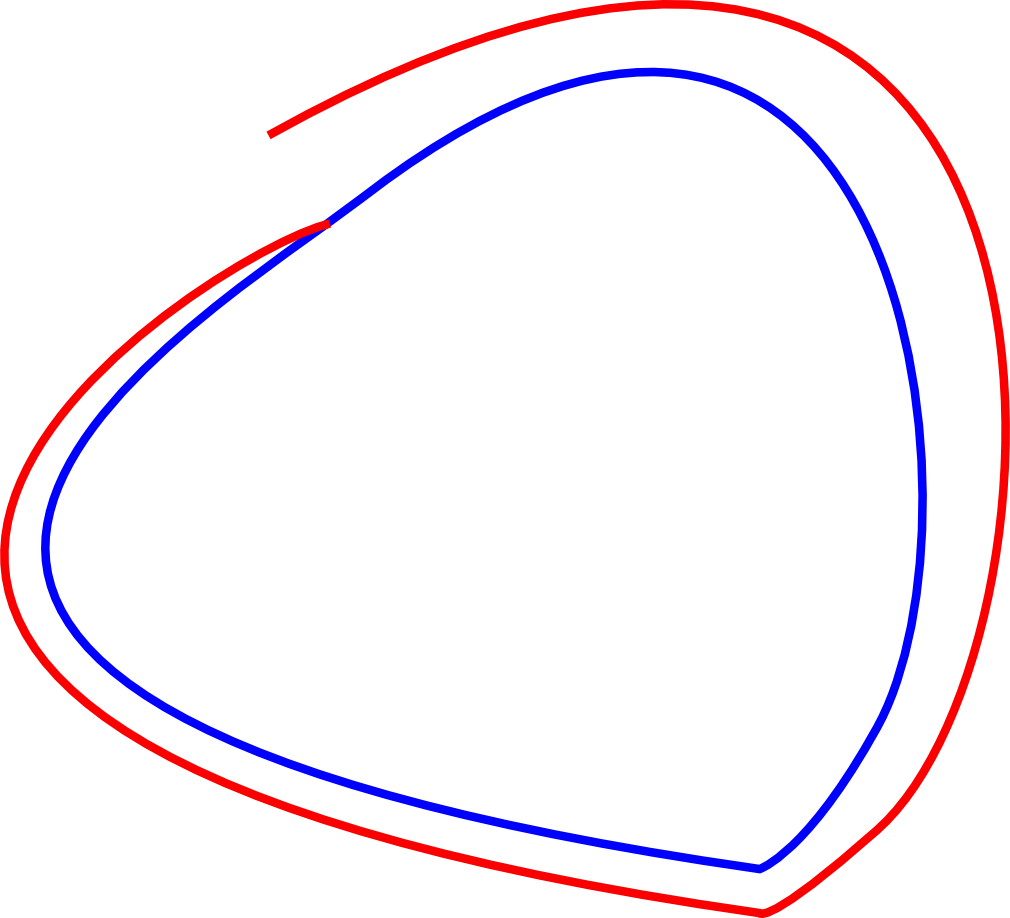
\includegraphics[scale=0.35]{images/drift}
\caption{Example of drift from real trajectory. Blue color: real camera trajectory, red color: estimation of trajectory with accumulated error.}
\end{center}
\end{figure}

\begin{figure}[!h]
\begin{center}
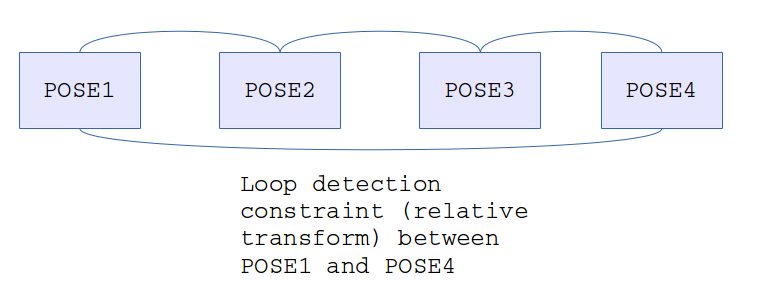
\includegraphics[scale=0.65]{images/loop_detection}
\caption{Example of loop closure constraint.}
\end{center}
\end{figure}

\subsubsection{Loop Detection}

In order to add loop closure constraints it is necessary to detect areas of the scene 
 that where previously visited. For this, images that have close euclidean distance between 
their corresponding poses are examined looking for similarities.

In order to detect previously visited areas of the scene SURF \cite{Bay06surf} feature detector 
is used. SURF keypoints are calculated and then the descriptors for each keypoint are obtained for 
each image.

 Then  the images are compared, using the difference between SURF descriptors.   


\section{Proposed Algorithm}
\begin{algorithmic}[1]
\State init R,t using Optical Flow
\State A = sobelFilter(A)
\State B = sobelFilter(B)
\State A' $\leftarrow$ transform(A,R,t) 
\State p $\leftarrow$ closestPoints(A',B)
\State $\{R,t\} \gets$ updateTransformation(p)
\State $e_i = meanSquareError(p)$
\If {$e_i < umbral$ OR  $i > maxIterations$} 
	\State return R,t
\Else
	\State goto step 4
\EndIf
\end{algorithmic}

The proposed algorithm uses optical flow to give a first estimation of 
R,t to the ICP algorithm. The used camera captures both depth and color 
information, for each pair of consecutive color captures optical flow 
is applied, obtaining pairs of correspondences between both captures. 

The domain of optical flow is on the 2D image space, but using 
the 3D information from the depthmap its possible to get the 3D position 
of the each pair of correspondences respect to the camera. 

Having pairs of 3D points, one point of the capture at time t and other point 
of the capture at time t + 1 its possible to obtain the rotation R and translation t
 that minimizes the distances between the correspondences. Obtaining the initial guess 
 for ICP.






\chapter{Results and Discussion}
\section{Dataset}

The dataset \cite{sturm12iros} was used to get a quantitative evaluation 
of the proposed solution. The dataset consists of 39 sequences recorded in
two different indoor environments. Each sequence contains
the color (RGB) and depth map images, as well as the ground truth
trajectory from a motion capture system and  evaluation 
scripts.

The dataset contains the Kinect parameters (image principal point and focal length), the timestamp of each RGB image and depth map, 
and scripts to associate RGB images to depth maps. This dataset is mainly used to test SLAM methods, where the 
interest is not only reconstruct the scene, but also know the trajectory of some moving vehicle equipped with
 sensors.

\section{Software and Hardware}

The software \cite{SourceCode} was programmed in C++ using Point Cloud Library (PCL), Open Computer Vision (OpenCV) and 
A General Framework for Graph Optimization (g2o).

\begin{itemize}

\item The Point Cloud Library (PCL) \cite{pcl} contains the ICP implementation used in this proposal.

\item OpenCV \cite{opencv} contains most common image processing algorithms and it was used to apply 
optical flow and SURF to images. 

\item $G_2$o library \cite{g2o}  was used to apply graph optimization.

\end{itemize}

The program was executed on a notebook with Ubuntu 13.10 Operating System, 
CPU Intel i5-3210M CPU @ 2.50GHz, 6 GB of RAM 
and a dedicated GPU Nvidia 650M of 2GB. Since software optimization is beyond of the scope 
of this thesis, no optimizations were performed and the software just used the CPU for the calculations.

\section{Evaluation Metrics}

The utilized dataset contains groundtruth sensor position and orientation along with two 
evaluation metrics: ATE (Absolute Trajectory Error) and RPE (Relative Pose Error). This metrics 
allows to estimate local and global error of the estimations compared to the provided grountruth measure. The dataset
 also provides the necessary tools to calculate the metrics. A detailed explanation can be found in \cite{sturm12iros}.

We have a sequence of poses from estimated trajectory $P_1,...,P_n \in SE(3)$ and from ground truth trajectory 
$Q_1,...,Q_n \in SE(3)$. Each pose represents global rotation and translation of the sensor.



\subsection{Relative Pose Error}

This error measure compares the groundtruth sensor trajectory in a fixed interval of time, frames, distance or degrees. 
Allowing for example to estimate how much error is produced frame to frame.

The relative pose error at time $i$ is defined as follows:

\begin{equation}
E_i = ( Q_i^{-1} Q_{i+\Delta})^{-1}(P_i^{-1}P_{i+\Delta})
\end{equation}

From these errors the root mean squared error (RMSE) is calculated over all time indices of the translational component as:

\begin{equation}
VRMSE(E_{1:n},\Delta) = (\frac{1}{m} \sum_{i=1}^m ||trans(E_i)||^2 )^{\frac{1}{2}}
\end{equation}


\subsection{Absolute Trajectory Error}

This error measure compares the groundtruth sensor trajectory with the proposed trajectory using root mean 
squared error and considering only translational errors. It is not necessary to consider the rotational components, 
because they are implicitly affecting sucesive sensor translations.

Since both trajectories can be in different coordinate frames, first they are aligned using the Horn method \cite{Horn}. If $S$ 
is the rigid-body transformation (obtained by least squares) that maps $P_{1:n}$ to $Q_{1:n}$, the absolute trajectory error
 at time step $i$ can be defined as follows:

\begin{equation}
F_i=Q_i^{-1}SP_i
\end{equation}

Then the root mean squared error over all time indices of the translational components can be defined as:

\begin{equation}
RMSE(F_{1:n}) = (\frac{1}{n} \sum_{i=1}^n ||trans(F_i)||^2 )^{\frac{1}{2}}
\end{equation}






\section{Results}
\subsection{Summary}

     The algorithm was tested using three different datasets from \cite{sturm12iros}. The main contribution of the 
proposal is the filtering method, removing points that are unlikely to be present in the two point clouds and are not 
near edges extracted from the RGB image. For this reason, experiments were conducted to compare the whole system performance 
with and without filtering. In the three datasets the proposed method with filtering has significantly better performance after 
graph optimization. System was tested using only 100 frames to maintain accumulated error low, outliers detection and a more advanced  
pose graph optimization setup is necessary to work with more frames, but this topic is beyond the scope of this thesis.

\subsection{Quantitative Results}
\begin{center}
\begin{table}[H]
\begin{tabular}{ |l|c|c|}
\hline & filtered point cloud & full point cloud \\
\pbox{20cm}{RPE \\ (RMSE per second)} & 0.303387 m & 0.273217 m \\
\hline
\pbox{20cm} {RPE after graph optimization \\ (RMSE per second)} &  0.066331 m &  0.114962 m\\
\hline
\pbox{20cm}{ATE \\ (RMSE)} & 0.103475 m & 0.078300 m\\
\hline
\pbox{20cm} {ATE after graph optimization \\ (RMSE)} & 0.040286 m & 0.061566 m\\
\hline
\end{tabular}
\caption{freiburg1\_desk dataset (first 100 frames).}
\label{table:quantfd1}
\end{table}
\end{center}


\begin{center}
\begin{table}[H]
\begin{tabular}{ |l|c|c|}
\hline & filtered point cloud & full point cloud \\
\pbox{20cm} {RPE \\ (RMSE per second)} & 0.124113 m & 0.158429 m \\
\hline
\pbox{20cm}{RPE after graph optimization \\ (RMSE per second)} & 0.081823 m & 0.112310 m\\
\hline
\pbox{20cm} {ATE \\ (RMSE)} & 0.059671 m & 0.078372 m\\
\hline
\pbox{20cm} {ATE after graph optimization \\ (RMSE)} & 0.048461 m & 0.063755 m\\
\hline
\end{tabular}
\caption{freiburg1\_room dataset (first 100 frames).}
\label{table:quantroom}
\end{table}
\end{center}

\begin{center}
\begin{table}[H]
\begin{tabular}{ |l|c|c|}
\hline & filtered point cloud & full point cloud \\
\pbox{20cm}{RPE \\ (RMSE per second)} &  0.044770 m & 0.105270 m\\
\hline
\pbox{20cm} {RPE after graph optimization \\ (RMSE per second)} & 0.041990 m & 0.114090 m\\
\hline
\pbox{20cm} {ATE \\ (RMSE)} & 0.025618 m  & 0.056300 m\\
\hline
\pbox{20cm} {ATE after graph optimization \\ (RMSE)} & 0.026500 m & 0.057818 m \\
\hline
\end{tabular}
\caption{freiburg2\_desk dataset (first 100 frames).}
\label{table:quantfd2}
\end{table}
\end{center}

\begin{center}
\begin{figure}
\begin{tikzpicture}[scale=1.5]
\begin{axis}[
    ybar,
    enlargelimits=0.15,
    legend style={at={(0.5,-0.15)},
      anchor=north,legend columns=-1},
    ylabel={execution time (minutes)},
    symbolic x coords={Fr1Desk,Fr2Desk,Fr1Room},
    xtick=data,
    nodes near coords,
    nodes near coords align={vertical},
    ]
\addplot coordinates {(Fr1Desk,15.16) (Fr2Desk,38.29) (Fr1Room,17.04)};
\addplot coordinates {(Fr1Desk,48.95) (Fr2Desk,344.32) (Fr1Room,116.49)};
\legend{filtered,non-filtered}
\end{axis}
\end{tikzpicture}
\caption{Average execution time with 100 frames in three different datasets} 
\end{figure}
\end{center}

In the freiburg1\_desk dataset before applying graph optimization better results where obtained using 
the full point cloud. This occurs because prior to graph optimization only consecutive frames are aligned, 
consecutive frames are more likely to have a small relative movement, making the alignment between two point clouds 
less prone to 
errors. When graph optimization is used, non consecutive frames are aligned in order to add restrictions to the graph, 
incrementing the difficulty of 
the alignment. Under this scenario the advantages of using the proposed filtering approach becomes clear.


\begin{figure}[H]
\begin{center}
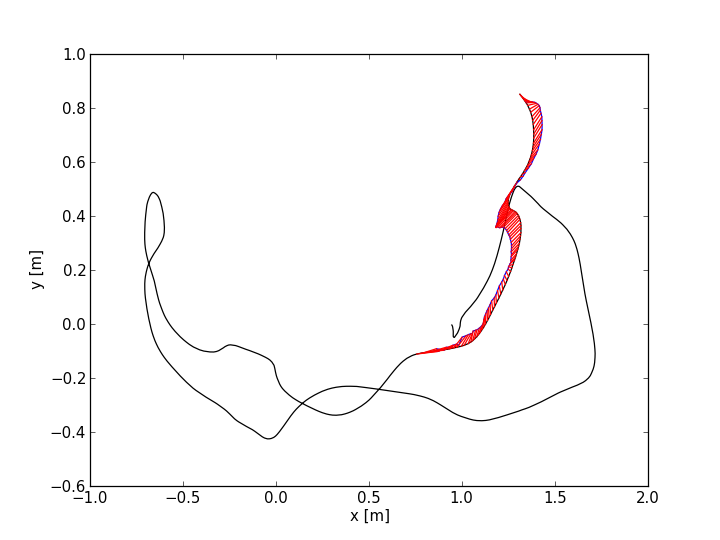
\includegraphics[scale=0.75]{images/freiburg1_desk_1_100_fullcloud_optimized.png}
\caption{freiburg1\_desk dataset first 100 frames: Obtained trajectory using full point cloud after graph optimization. Ground truth trajectory (black), estimated trajectory (blue) and difference (red).}
\end{center}
\end{figure}

\begin{figure}[H]
\begin{center}
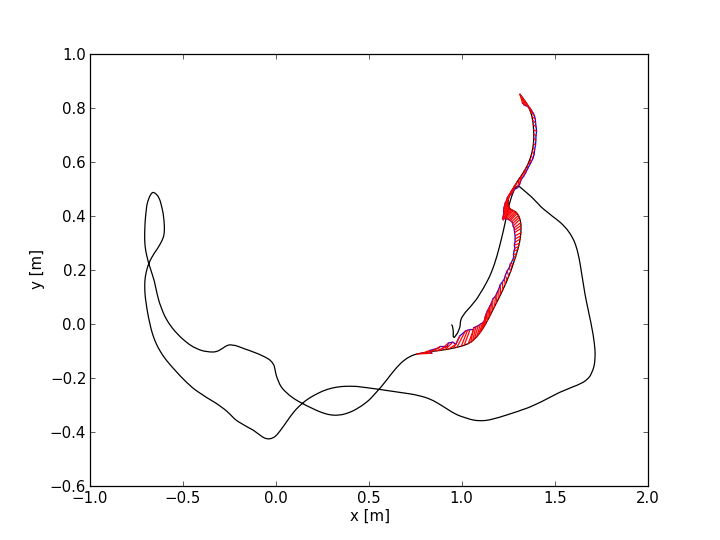
\includegraphics[scale=0.75]{images/freiburg1_desk_1_100_optimized.png}
\caption{freiburg1\_desk dataset first 100 frames: Obtained trajectory using point cloud filtered with proposed method after graph optimization. Ground truth trajectory (black), estimated trajectory (blue) and difference (red).}
\end{center}
\end{figure}

\begin{figure}[H]
\begin{center}
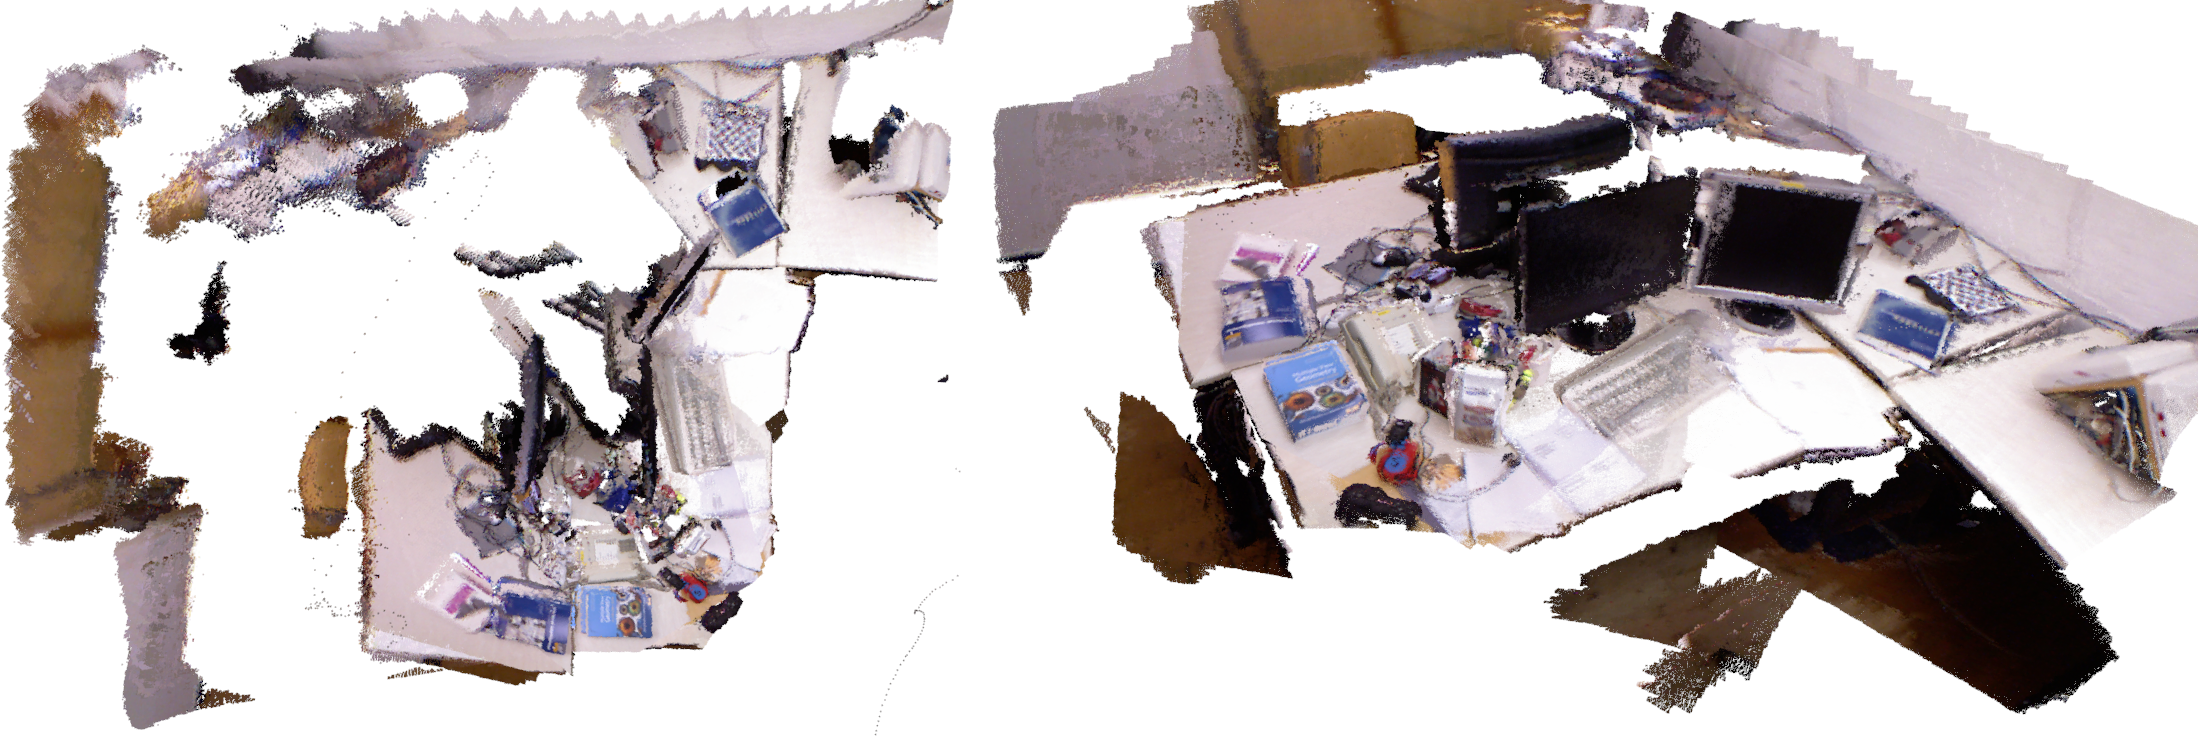
\includegraphics[scale=0.2]{images/freiburg1_desk.png}
\caption{freiburg1\_desk dataset registration of first 100 frames with proposed method. Point cloud downsampled using voxels of $35mm$.}
\end{center}
\end{figure}


\begin{figure}[H]
\begin{center}
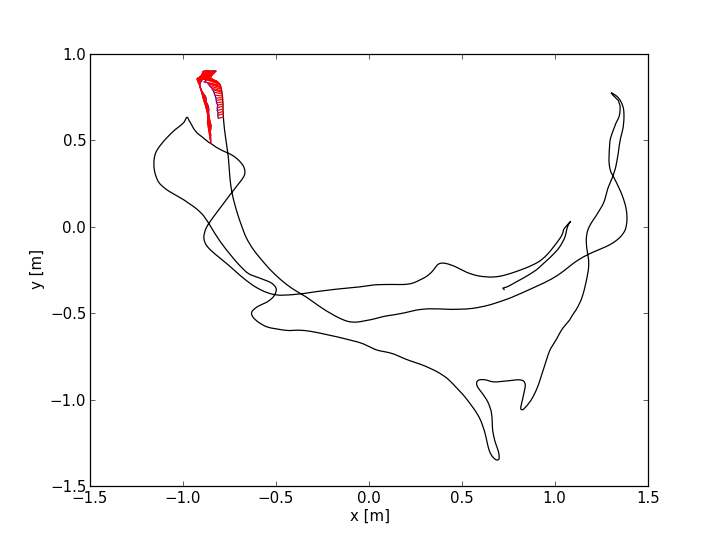
\includegraphics[scale=0.75]{images/freiburg1_room_1_100_fullcloud_optimized.png}
\caption{freiburg1\_room dataset first 100 frames: Obtained trajectory using full point cloud after graph optimization. Ground truth trajectory (black), estimated trajectory (blue) and difference (red).}
\end{center}
\end{figure}

\begin{figure}[H]
\begin{center}
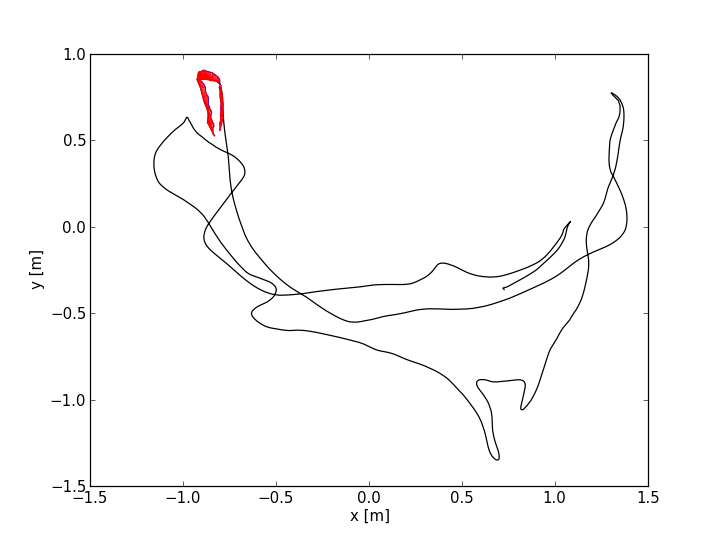
\includegraphics[scale=0.75]{images/freiburg1_room_1_100_optimized.png}
\caption{freiburg1\_room dataset first 100 frames: Obtained trajectory using point cloud filtered with proposed method after graph optimization. Ground truth trajectory (black), estimated trajectory (blue) and difference (red).}
\end{center}
\end{figure}

\begin{figure}[H]
\begin{center}
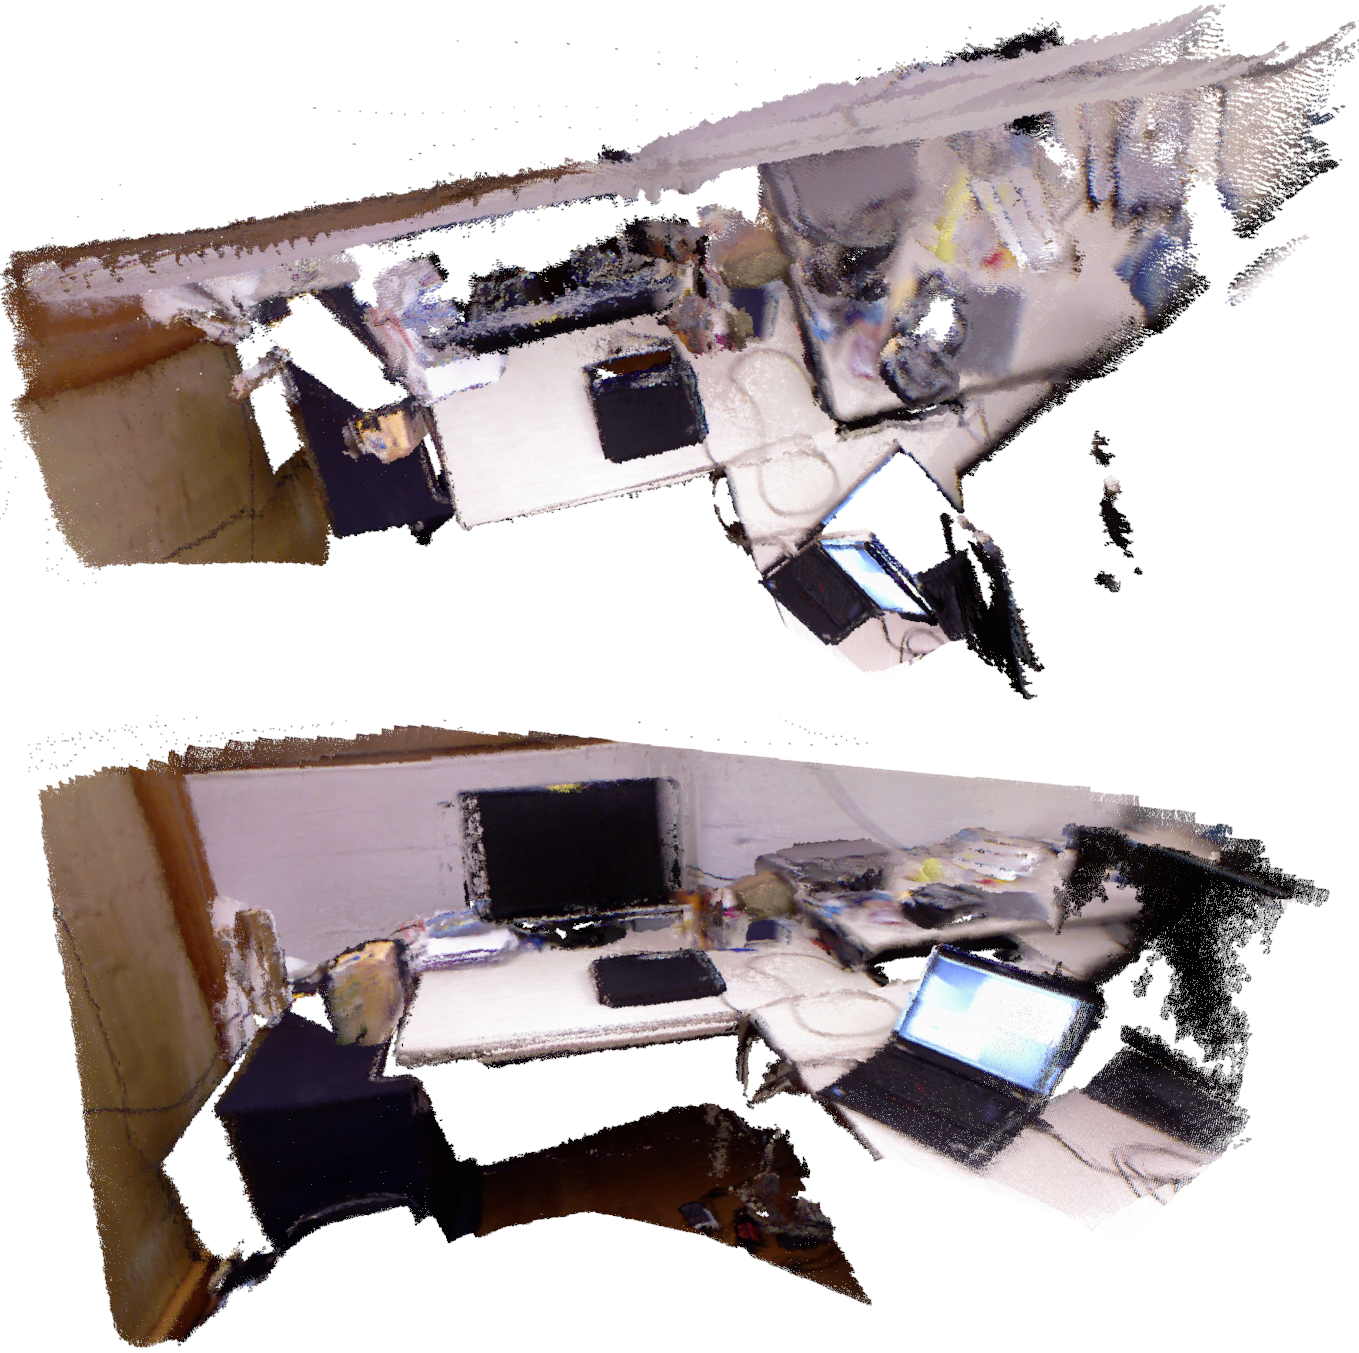
\includegraphics[scale=0.27]{images/freiburg1_room.png}
\caption{freiburg1\_room dataset registration of first 100 frames with proposed method. Point cloud downsampled using voxels of $35mm$.}
\end{center}
\end{figure}


\begin{figure}[H]
\begin{center}
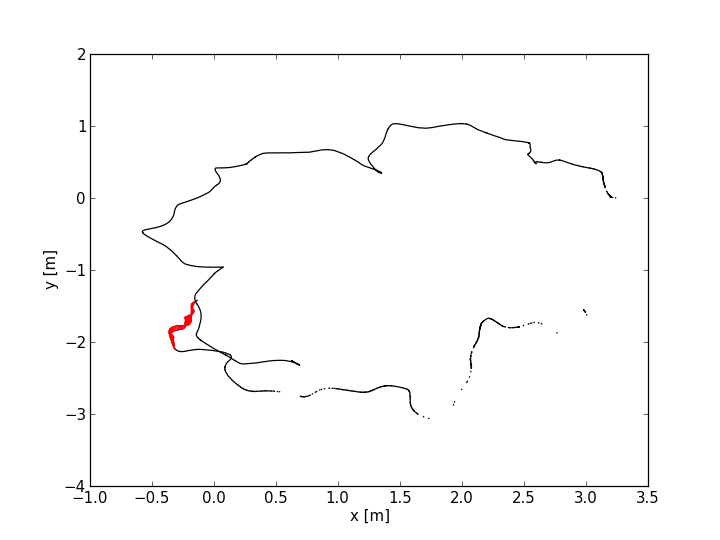
\includegraphics[scale=0.75]{images/freiburg2_desk_1_100_fullcloud_optimized.png}
\caption{freiburg2\_desk dataset first 100 frames: Obtained trajectory using full point cloud after graph optimization. Ground truth trajectory (black), estimated trajectory (blue) and difference (red).}
\end{center}
\end{figure}

\begin{figure}[H]
\begin{center}
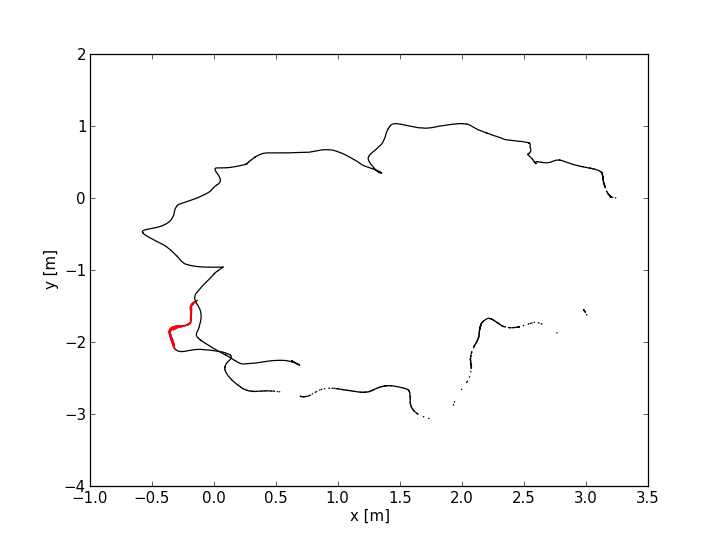
\includegraphics[scale=0.75]{images/freiburg2_desk_1_100_optimized.png}
\caption{freiburg2\_desk dataset first 100 frames: Obtained trajectory using point cloud filtered with proposed method after graph optimization. Ground truth trajectory (black), estimated trajectory (blue) and difference (red).}
\end{center}
\end{figure}


\begin{figure}[H]
\begin{center}
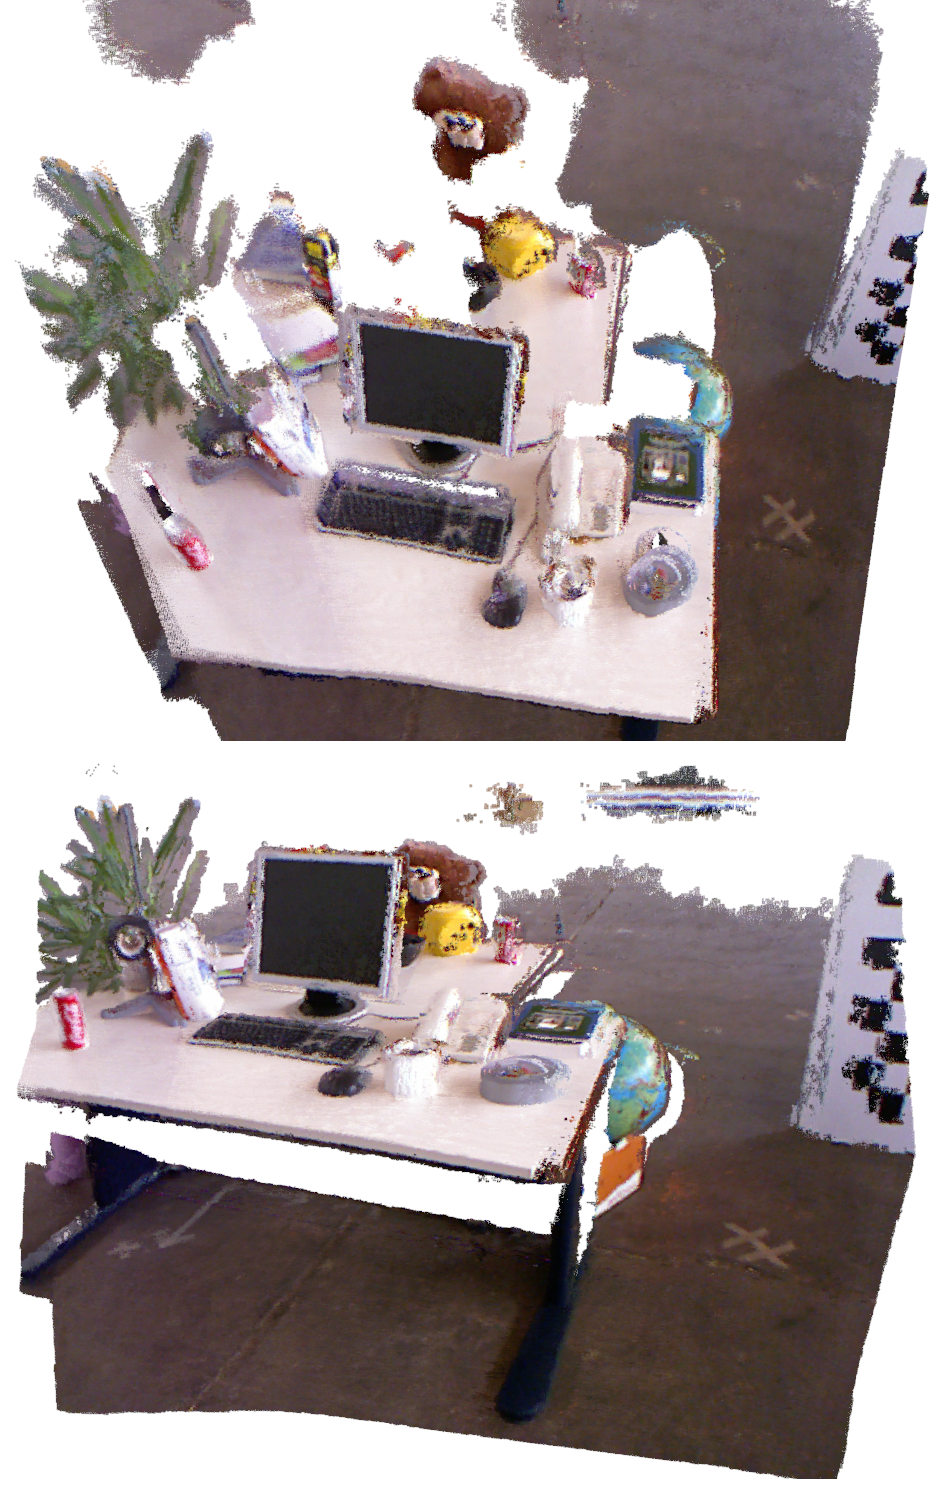
\includegraphics[scale=0.27]{images/freiburg2_desk.png}
\caption{freiburg2\_desk dataset registration of first 100 frames with proposed method. Point cloud downsampled using voxels of $55mm$.}
\end{center}
\end{figure}


As it can be seen in previous plots, when applying the proposed filtering to the point clouds, the estimated trajectory of the sensor gets 
closer to ground truth. Better results are obtained working with a representative small subset of the original data and these results 
can be greatly improved with a better setup of the pose graph. Reconstructed scenes shown the potential of the method and the quantitative 
results can be verified through a visual inspection. 

The best results where obtained in the freiburg2\_desk dataset, possibly due to the visual richness of the images more clues where obtained 
to find the relative transformations.

%\chapter{Point Features}
%\index{Point Features}
%
A point feature is some characteristic that identifies the point and is desirable 
that points with geometrical similarities share similar features. For example..

\section{Point Neighboorhood}

In order to talk about point features is necessary to define a neighboorhood. 

We will define a neighboordhood of a point as a set of points that are related 
with it, sharing some common properties.

k neightboorhood : the k closests points 

radious neightboorhood : all the points that are within some radious

\section{Point Normal}

A very important geometrical property of a point is the normal. 
Because it indicates the orientation of the surface that contains it,
this property is heavily used in computer graphics to compute the 
lighting of an scene, since with the normals we can simulate the 
trajectory of an light ray that is intersecting the surface.
This property is also used as a point feature.



\section{Point Curvature}

The curvature is related with normal changes in a surface, 
a surface with no curvature will have all the normals pointing 
to the same direction. 




%\chapter{RGB Tracking}
%\index{RGB Tracking}

\chapter{Conclusions}
\label{conclusions}
\index{Conclusions}


This thesis provides a registration algorithm that uses geometrical and visual information 
to perform the alignment between RGB-D frames.  

A first estimation of the relative transformation between each pair of successive frames was obtained using 
visual information, with optical flow and SURF methods. An edge filtering technique was applied to detect a representative subset 
of the data, using only between 10\% and 20\% of original points as input to ICP algorithm. Finally a pose graph optimization method increases overall result quality.

The proposed algorithm reduces the execution time and takes advantage of rich textured surfaces to align point clouds. The edge filtering technique removes flat surfaces with poor visual clues, taking advantage of the RGB images captured by the sensor in order to filter the point clouds, working with a representative subset in order to increase the alignment quality.


Promising results were obtained using a freely available dataset. The method was evaluated quantitatively and 
also some images of the 3D reconstructed scenes were obtained for a visual inspection of the results.

\section{Future Work}

  Results can be greatly improved adding an outlier detection method, because one incorrect align between two frames can ruin the complete result. These problems can occur 
when one of the frames exhibit poor visual features or there is an abrupt change in the sensor movement. 

  Another important part of the system that can be improved is the pose graph, where the quality of the restrictions 
determines the quality of the end result. For example, removing some restrictions and adding restrictions obtained with a 
different alignment method or performing some parameter tunning of the proposed method, in 
order to obtain better relative alignment when certain conditions are satisfied.



\appendix
\addcontentsline{toc}{chapter}{Appendix}
\chapter{Trace Lemma}
\label{ap:lemma}
\begin{mybox}{gray}{Lemma}
For any positive definite matrix $A A^t$ and any orthogonal matrix B 

\[ Trace( A A^t ) \geq Trace (B A A^t) \]

\end{mybox}


Proof of lemma:

Let $a_i$ be the ith column of A, then:

\begin{align*}
Trace( B A A^t ) = Trace (A^t B A) = \sum\limits_i a_i^t B a_i 
\end{align*}

But by the Schwarz inequality

\[ a_i^t B a_i \leq \sqrt{ a_i^t a_i (a^t B^t B a_i)} = a^t a_i \]


\chapter{Acronyms}
\label{acronyms}
\index{acronyms}
\begin{description}
\item ICP: Iterative Closest Point 
\end{description}
%%%%%%%%%%%%%%%%%%%%%%%%%%%%%%%%%%%%%%%%%%%%%%%%%%%%%%%%%%%%%%%%%%%
%\begin{com}
%Aqui estaba la seccion que yo echaba de menos.
%Convendria indicar todas las paginas/lineas en que aparece referido
%cada acronimo o, quizas, solo la primera vez que aparece.
%¿Tiene \LaTeXe\ un mecanismo automatico para hacer esto?

%\textcolor{red}{Se puede referenciar a las secciones, no se si
%  especificamente a cada item, voy a estudiarlo.}

%¿ESTA COMPLETA LA LISTA DE ACRONIMOS?
%\end{com}
%%%%%%%%%%%%%%%%%%%%%%%%%%%%%%%%%%%%%%%%%%%%%%%%%%%%%%%%%%%%%%%%%%%


%\begin{figure}[htbp]
%\centering
%\epsfig{file=figura.eps,scale=0.5}
%\caption{}
%\label{fig:esquema1}
%\end{figure}

%\begin{Verbatim}[commandchars=\\\\?,frame=single,fontsize=\relsize{-2 }]
      
%\begin{table}[h!tpb]  
%\begin{center}
%\begin{tabularx}{450pt}{|>{\hsize=0.5\hsize}X|>{\hsize=0.5\hsize}X|}
%\hline

% & \\ \hline

%\end{tabularx}
%\end{center}
%\caption{Curso Normal de Eventos Inscripcin.}
%\end{table}
%\addcontentsline{toc}{chapter}{\bibname}		  
 		  

%\begin{thebibliography}{99}
%\bibitem{uno} Apellido, Nombre del Autor
 % ``Titulo''.
 % Descripcin, Ao.

%\bibitem{dos} Ms referencias \url{http://www.google.cl}

%\end{thebibliography}


%%%%%%%%%%%%%%%%%%%%%%%%%%%%%%%%%%%%%%%%%%%%%%%%%%%%%%%%%%%%%%%%%%%%%
%\begin{com}
%NO HAY BIBLIOGRAFIA HASTA AHORA (15.05.2008)
%\end{com}
%%%%%%%%%%%%%%%%%%%%%%%%%%%%%%%%%%%%%%%%%%%%%%%%%%%%%%%%%%%%%%%%%%%%%

%%%%%%%%%%%%%%%%%%%%%%%%%%%%%%%%%%%%%%%%%%%%%%%%%%%%%%%%%%%%%%%%%%%
%\begin{com}
%Llevar control de versiones con fechas!!!
%\end{com}
%%%%%%%%%%%%%%%%%%%%%%%%%%%%%%%%%%%%%%%%%%%%%%%%%%%%%%%%%%%%%%%%%%%


%%%%%%%%%%%%%%%%%%%%%%%%%%%%%%%%%%%%%%%%%%%%%%%%%%%%%%%%%%%%%%%%%%%
%\begin{com}
%Aquí voy.  File procesado. Valpo., 15.05.2008
%\end{com}
%%%%%%%%%%%%%%%%%%%%%%%%%%%%%%%%%%%%%%%%%%%%%%%%%%%%%%%%%%%%%%%%%%%

\vspace{\fill}\LaTeXe





\backmatter

\addcontentsline{toc}{chapter}{\bibname}
\bibliographystyle{unsrt}
\bibliography{tesis}

\end{document}

